% =================================================================
% DOCUMENTO PRINCIPAL (main.tex)
% =================================================================
\documentclass[10pt,a4paper,twocolumn]{article}

% --- PACOTES DE LAYOUT E MARGENS ---
\usepackage[top=1.2cm, bottom=2.0cm, left=1.5cm, right=1.5cm, headheight=46pt, headsep=0.4cm, includehead]{geometry}

% --- PACOTES DE IDIOMA E FONTE ---
\usepackage[T1]{fontenc}               % Codificação de fonte vetorial
\usepackage[utf8]{inputenc}            % Suporte a acentuação
\usepackage[brazilian]{babel}          % Idioma em português do Brasil
\usepackage{newtxtext, newtxmath}      % Fonte padrão Times (texto e matemática)
\usepackage{parskip} % já aplica o padrão moderno automaticamente (~6pt de espaço e 0pt de recuo)


% --- PACOTES GRÁFICOS, TABELAS E LISTAS ---
\usepackage{graphicx}                  % Inclusão de imagens e logos
\usepackage{booktabs}                  % Tabelas limpas
\usepackage{float}                     % Controle de posição de figuras
\usepackage{enumitem}                  % Suporte estendido a listas (itemize/enumerate)
\setlist{nosep, leftmargin=*}

% --- CRIAÇÃO DO AMBIENTE PERSONALIZADO "GRAFICO" ---
\usepackage{newfloat}
\DeclareFloatingEnvironment[
    fileext=log,
    listname={Lista de Gráficos},
    name=Gráfico,
    placement=htbp,
]{grafico}

% --- PACOTES MATEMÁTICOS E UNIDADES ---
\usepackage{amsmath, amsfonts}         % Equações e símbolos básicos
\let\Bbbk\undefined                    % Evita conflito do símbolo \Bbbk
\usepackage{amssymb}                   % Símbolos matemáticos adicionais
\usepackage{siunitx}                   % Formatação de unidades
\sisetup{output-decimal-marker = {,}}

% --- PACOTES DE DESENHO E CIRCUITOS ---
\usepackage{tikz}
\usepackage[american]{circuitikz}

% --- PACOTES DE CITAÇÃO E LINKS ---
\usepackage{cite}                      % Citações numéricas
\usepackage{xurl}                      % Quebra de linha em URLs
\usepackage[hidelinks]{hyperref}       % Links invisíveis e metadados no PDF

% --- PACOTES DE CABEÇALHO E TIPOGRAFIA ---
\usepackage{fancyhdr}                  % Cabeçalhos e rodapés customizados
\usepackage[expansion=false]{microtype}% Ajuste tipográfico
\usepackage{caption}
\usepackage{subcaption}                % Suporte para o ambiente subfigure

% --- CONFIGURAÇÕES DE FLUTUAÇÃO DE IMAGENS E LEGENDAS ---
\raggedbottom                          
\setlength{\floatsep}{6pt plus 2pt minus 2pt}      
\setlength{\textfloatsep}{8pt plus 2pt minus 2pt}  
\setlength{\intextsep}{6pt plus 2pt minus 2pt}     
\setlength{\abovecaptionskip}{4pt}                 
\setlength{\belowcaptionskip}{2pt}                 
\captionsetup{skip=3pt}

% --- CONFIGURAÇÕES DE PÁGINA ---
\pagestyle{fancy}

% --- INÍCIO DO DOCUMENTO ---
\begin{document}

% Inclusão das configurações de página e informações do título
\fancyhf{} % Limpa todos os cabeçalhos e rodapés atuais

% --- CABEÇALHO PADRÃO PARA TODAS AS PÁGINAS ---
\lhead{$\vcenter{\hbox{
\includegraphics[height=1.4cm]{Heading/Logo_CI_Inovador.png}}}$\vspace{6pt}}
\rhead{$\vcenter{\hbox{
\includegraphics[height=1.4cm]{Heading/Logo_UFPR.png}}}$\vspace{6pt}}

% --- RODAPÉ ---
\lfoot{\small Curso de Especialização em Microeletrônica - Lato Sensu -- UFSM -- Polo UFPR GICS}
\rfoot{\small Página \thepage}

\renewcommand{\headrulewidth}{0.4pt}
\renewcommand{\footrulewidth}{0.4pt}

% --- REDEFINIÇÃO DO ESTILO PLAIN (PRIMEIRA PÁGINA) ---
\fancypagestyle{plain}{
  \fancyhf{}
  \lhead{$\vcenter{\hbox{
\includegraphics[height=1.4cm]{Heading/Logo_CI_Inovador.png}}}$\vspace{6pt}}
  \rhead{$\vcenter{\hbox{
\includegraphics[height=1.4cm]{Heading/Logo_UFPR.png}}}$\vspace{6pt}}
  \lfoot{\small Curso de Especialização em Microeletrônica - Lato Sensu -- UFSM -- Polo UFPR GICS}
  \rfoot{\small Página \thepage}
  \renewcommand{\headrulewidth}{0.4pt}
  \renewcommand{\footrulewidth}{0.4pt}
}
\title{\textbf{Lab - 1}}
\author{
  \textbf{Jose Guilherme Elizeire Mendina Junior}\\
  \small Programa de Formação e Residência em Microeletrônica -- CI Inovador\\
  \small Curso de Especialização em Microeletrônica - Lato Sensu -- UFSM -- Polo UFPR\\
  \small \texttt{guilherme.mendina@acad.ufsm.br} | \texttt{guilherme.mendina@ufpr.br}\\
  \small Disciplina: Amplificadores 2 \\
}
\date{\today}

\maketitle
\thispagestyle{plain}
\setlength{\parindent}{0pt}

% Conteúdo do artigo
\section{Introdução}
\label{sec:introducao}
Filtros analógicos são circuitos eletrônicos essenciais no processamento de sinais, projetados para selecionar faixas de frequência específicas enquanto atenuam sinais interferentes indesejados \cite{razavi2006fund}. Em sistemas de comunicação sem fio e telefonia móvel, essa seletividade é crítica: receptores operam em ambientes congestionados e precisam isolar o canal de interesse de ruídos e interferências de bandas adjacentes antes que o sinal seja processado \cite{razavi2006fund}.

Diferentemente de aplicações em baixa frequência — como a filtragem de ruído da rede elétrica ($50\text{ Hz}$ ou $60\text{ Hz}$) em sinais de áudio —, o projeto de filtros em Radiofrequência (RF) exige que o fluxo do sinal seja tratado em termos de potência. Nessa faixa de operação, o comprimento de onda torna-se comparável às dimensões dos componentes, tornando indispensável o casamento de impedância (padronizado em $50~\Omega$) para garantir a máxima transferência de potência, minimizar perdas de inserção (\textit{insertion loss}) e evitar distorções de fase \cite{ludwig2000rf}.

Projetar filtros de alta frequência diretamente do zero torna-se matematicamente complexo à medida que a ordem aumenta, exigindo um método sistemático passo a passo \cite{ludwig2000rf}. Inicialmente, define-se a categoria de filtragem adequada à aplicação — passa-baixas (\textit{low-pass}), passa-altas (\textit{high-pass}), passa-faixa (\textit{bandpass}) ou rejeita-faixa (\textit{bandstop}) — partindo-se de um protótipo passa-baixas normalizado. Em seguida, seleciona-se a função de aproximação mais apropriada, como Butterworth ou Chebyshev, bem como a ordem do filtro ($N$), que determinam o compromisso entre a seletividade e o comportamento na banda passante, além da quantidade e distribuição dos elementos reativos. Por fim, os coeficientes normalizados são submetidos à desnormalização de impedância e à transformação em frequência para adequar os valores dos componentes à faixa de operação desejada \cite{ludwig2000rf}.

O relatório apresenta o dimensionamento e a validação computacional de um filtro passa-faixa de quinta ordem ($N = 5$) baseado na aproximação de Chebyshev, destinado a um receptor operando na frequência central de $f_0 = 6,5\text{ GHz}$ com largura de banda de $BW = 500\text{ MHz}$ (espectro de $6,25\text{ GHz}$ a $6,75\text{ GHz}$) e impedâncias terminais de $50~\Omega$, seguindo as especificações estabelecidas no roteiro da atividade \cite{Filter1}.

A escolha dessa faixa de operação fundamenta-se na sua relevância estratégica para os sistemas sem fio de alta capacidade e curto alcance. Por um lado, uma portadora em torno de $6,5\text{ GHz}$ com largura de banda de $500\text{ MHz}$ é característica de aplicações \textit{Ultra-Wideband} (UWB) — a exemplo do Canal 5 do padrão IEEE 802.15.4, centrado em aproximadamente $6,49\text{ GHz}$ —, nas quais o amplo espectro permite a transmissão de pulsos de curtíssima duração e elevada resolução temporal para localização precisa (ordem de centímetros), sensoriamento, radares de curto alcance e comunicação veicular (V2X) em veículos conectados \cite{ieee802154}. Nessa região de frequência, a maior atenuação por obstáculos favorece enlaces locais de alta taxa e precisão em detrimento de comunicações de longa distância.

Por outro lado, a banda de $6\text{ GHz}$ ($5,925\text{ GHz}$ a $7,125\text{ GHz}$) insere-se diretamente no atual cenário regulatório de compartilhamento espectral entre redes locais de alta velocidade e serviços móveis. No Brasil, a Agência Nacional de Telecomunicações (Anatel), por meio do Acórdão nº~203 e do Ato nº~10.400 de agosto de 2026, destinou oficialmente a subfaixa inferior de $5,925\text{ GHz}$ a $6,425\text{ GHz}$ ($500\text{ MHz}$ de largura) para equipamentos de radiação restrita (Wi-Fi 6E e Wi-Fi 7), mantendo os $700\text{ MHz}$ superiores ($6,425\text{ GHz}$ a $7,125\text{ GHz}$) alocados ao Serviço Móvel Pessoal (5G/6G), em consonância com a norma europeia ETSI EN 303 687 e as diretrizes da WRC-23 da UIT \cite{anatel2026ato10400, etsi303687}. Operar em $f_0 = 6,5\text{ GHz}$ posiciona o receptor exatamente nessa fronteira crítica de transição espectral, tornando rigoroso o requisito de atenuação mínima de $25\text{ dB}$ a partir de $1,5 \times BW$ para suprimir interferências de canais móveis adjacentes \cite{Filter1}.


\section{Metodologia}

A atividade seguiu o procedimento proposto no roteiro \cite{Filter1}, dividindo-se nas etapas de síntese analítica, a definição da ordem do filtro, implementação do esquemático e validação computacional no ambiente \textit{Cadence Virtuoso} (ADE Maestro). Conforme as instruções especificadas, utilizaram-se componentes ideais das bibliotecas \texttt{analogLib} e \texttt{rfLib}, garantindo o casamento de impedância em $Z_0 = 50~\Omega$ nas portas de entrada e saída.


\subsection{Dimensionamento e Implementação Esquemática do Filtro}

Para o dimensionamento dos elementos, definiu-se primeiramente a frequência central de $f_0 = 6,5\text{ GHz}$ com largura de banda $BW = 500\text{ MHz}$, cuja motivação foi apresentada na Seção~\ref{sec:introducao}, seguindo as especificações estabelecidas no roteiro \cite{Filter1}.

Com base nos slides da aula \cite{schuartz2026slides}, a partir das informações contidas na Tabela~\ref{Tab:tabela1}, extraíram-se os coeficientes normalizados de quinta ordem ($N = 5$), resumidos na Tabela~\ref{tab:coeficientes_chebyshev}, para realizar os cálculos de dimensionamento dos componentes.

\begin{table}[htbp]
    \centering
    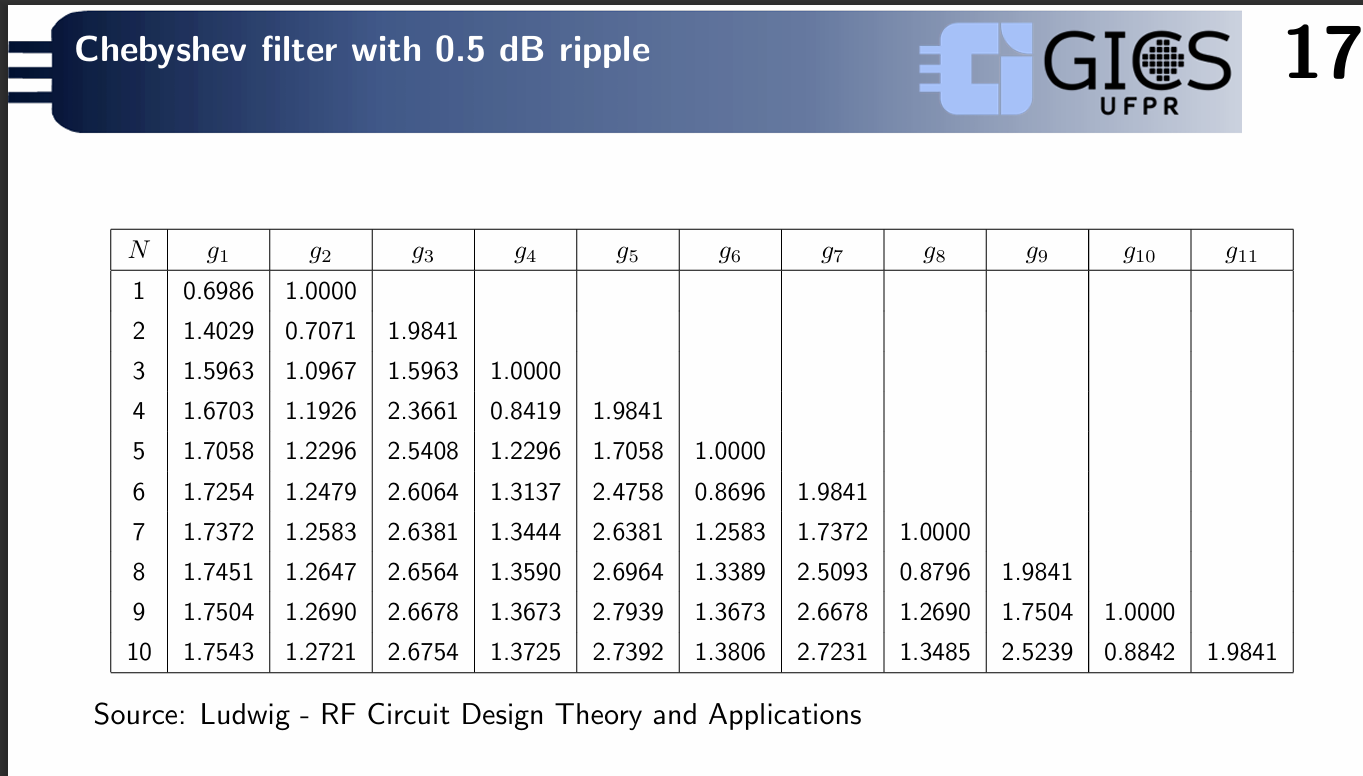
\includegraphics[width=\columnwidth]{Method/Fig/tabela1.png}
    \caption{Tabela de coeficientes normalizados para filtro Chebyshev com $0,5\text{ dB}$ de \textit{ripple} \cite{schuartz2026slides, ludwig2000rf}.}
    \label{Tab:tabela1}
\end{table}

\begin{table}[htbp]
    \centering
    \footnotesize
    \caption{Coeficientes normalizados do protótipo passa-baixas Chebyshev ($0,5\text{ dB}$ de \textit{ripple}, $N = 5$) \cite{ludwig2000rf, schuartz2026slides}.}
    \label{tab:coeficientes_chebyshev}
    \begin{tabular}{cccccc}
        \hline
        \textbf{$N$} & \textbf{$g_1$} & \textbf{$g_2$} & \textbf{$g_3$} & \textbf{$g_4$} & \textbf{$g_5$} \\
        \hline
        5 & $1,7058$ & $1,2296$ & $2,5408$ & $1,2296$ & $1,7058$ \\
        \hline
    \end{tabular}
\end{table}



Com valores obtidos na tabela \ref{tab:coeficientes_chebyshev}, foram realizado os calculos de dimensionamento para determinar os valore a seres atribuídos a cada componente:

\begin{align}
    f_L &= f_0 - \frac{BW_{\text{Hz}}}{2} = 6,25\text{ GHz} \\
    f_U &= f_0 + \frac{BW_{\text{Hz}}}{2} = 6,75\text{ GHz} \\
    \omega_0 &= 2\pi f_0 \approx 4,0841 \times 10^{10}\text{ rad/s} \\
    BW_{\text{rad}} &= 2\pi BW_{\text{Hz}} \approx 3,1416 \times 10^{9}\text{ rad/s}
\end{align}

Em seguida, realiza-se a desnormalização de impedância do protótipo passa-baixas para $R_G = 50~\Omega$, multiplicando os elementos indutivos ímpares ($g_1, g_3, g_5$) por $R_G$ e dividindo os elementos capacitivos pares ($g_2, g_4$) por $R_G$:
\begin{align}
    \tilde{L}_1 &= \tilde{L}_5 = g_1 R_G = 85,29\text{ H} \\
    \tilde{C}_2 &= \tilde{C}_4 = \frac{g_2}{R_G} = 24,592\text{ mF} \\
    \tilde{L}_3 &= g_3 R_G = 127,04\text{ H}
\end{align}

Por fim, aplica-se a transformação em frequência de passa-baixas para passa-faixa. Para os estágios série ($k = 1, 3, 5$), os valores dos indutores e capacitores são dados por:
\begin{align}
    L_1 &= L_5 = \frac{\tilde{L}_1}{BW_{\text{rad}}} = 27,15\text{ nH} \\
    C_1 &= C_5 = \frac{BW_{\text{rad}}}{\omega_0^2 \tilde{L}_1} = 22,08\text{ fF} \\
    L_3 &= \frac{\tilde{L}_3}{BW_{\text{rad}}} = 40,44\text{ nH} \\
    C_3 &= \frac{BW_{\text{rad}}}{\omega_0^2 \tilde{L}_3} = 14,83\text{ fF}
\end{align}

Para os estágios em paralelo (\textit{shunt}, $k = 2, 4$), os componentes ressonantes são obtidos por:
\begin{align}
    C_2 &= C_4 = \frac{\tilde{C}_2}{BW_{\text{rad}}} = 7,828\text{ pF} \\
    L_2 &= L_4 = \frac{BW_{\text{rad}}}{\omega_0^2 \tilde{C}_2} = 76,59\text{ pH}
\end{align}



Com os  valores dos componentes etao  resumidos na Tabela~\ref{tab:components}, 

\begin{table}[htbp]
    \centering
    \footnotesize
    \caption{Valores dimensionados dos componentes do filtro passa-faixa ($f_0 = 6,5\text{ GHz}$, $BW = 500\text{ MHz}$) e correspondência com o esquemático.}
    \label{tab:components}
    \begin{tabular}{cccc}
        \hline
        \textbf{Estágio ($k$)} & \textbf{Esquemático} & \textbf{Indutor} & \textbf{Capacitor} \\
        \hline
        1 (Série)    & \texttt{L0, C0} & $27,15\text{ nH}$ & $22,08\text{ fF}$ \\
        2 (Paralelo) & \texttt{L1, C1} & $76,59\text{ pH}$ & $7,828\text{ pF}$ \\
        3 (Série)    & \texttt{L2, C2} & $40,44\text{ nH}$ & $14,83\text{ fF}$ \\
        4 (Paralelo) & \texttt{L3, C3} & $76,59\text{ pH}$ & $7,828\text{ pF}$ \\
        5 (Série)    & \texttt{L4, C4} & $27,15\text{ nH}$ & $22,08\text{ fF}$ \\
        \hline
    \end{tabular}
\end{table}

 A modelagem do circuito do filtro foi implementada no \textit{Cadence Virtuoso}, conforme mostrado na Figura~\ref{fig:filtro_uwb_6g5}.


 \begin{figure}[htbp]
    \centering
    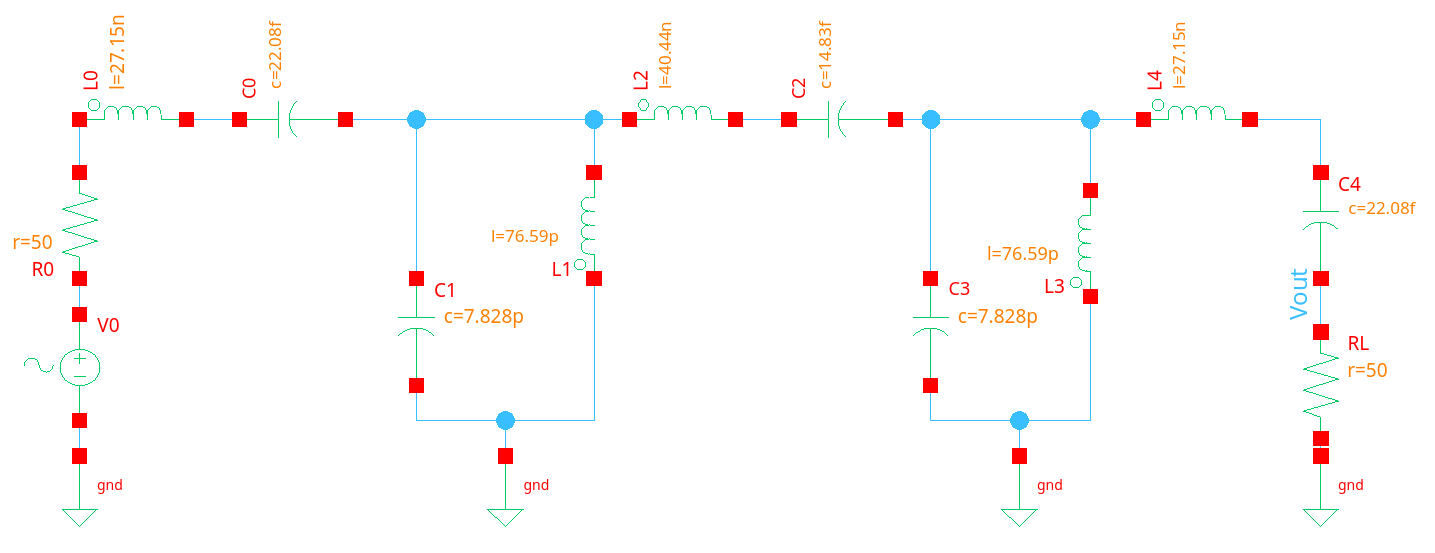
\includegraphics[width=\columnwidth]{Method/Fig/filtro_uwb_6g5.png}
    \caption{Esquemático do filtro passa-faixa UWB em $6,5\text{ GHz}$ implementado no \textit{Cadence Virtuoso}.}
    \label{fig:filtro_uwb_6g5}
\end{figure}
\section{Resultados}

\subsection{Resposta em Frequência (AC) e Análise de Polos e Zeros}

A magnitude linear da tensão de saída $V_{\text{out}}$ (\texttt{/net10}), obtida por meio da simulação AC, está representada na Figura~\ref{fig:ac_mag_lin}. Com essa análise, foi possível observar a característica \textit{equiripple} da aproximação de Chebyshev de quinta ordem ($N=5$), evidenciada pelos cinco picos máximos de aproximadamente $500\text{ mV}$ ($499{,}63\text{ mV}$ em $6{,}267\text{ GHz}$ e $499{,}42\text{ mV}$ em $6{,}743\text{ GHz}$) dentro da banda passante ($6{,}25\text{ GHz}$ a $6{,}75\text{ GHz}$). Esse valor corresponde à metade da amplitude da fonte ($1\text{ V}$), comprovando a ausência de perdas dissipativas nos elementos reativos ideais e o casamento de impedância entre $R_0 = 50~\Omega$ e $R_L = 50~\Omega$.

\begin{figure}[!htbp]
    \centering
    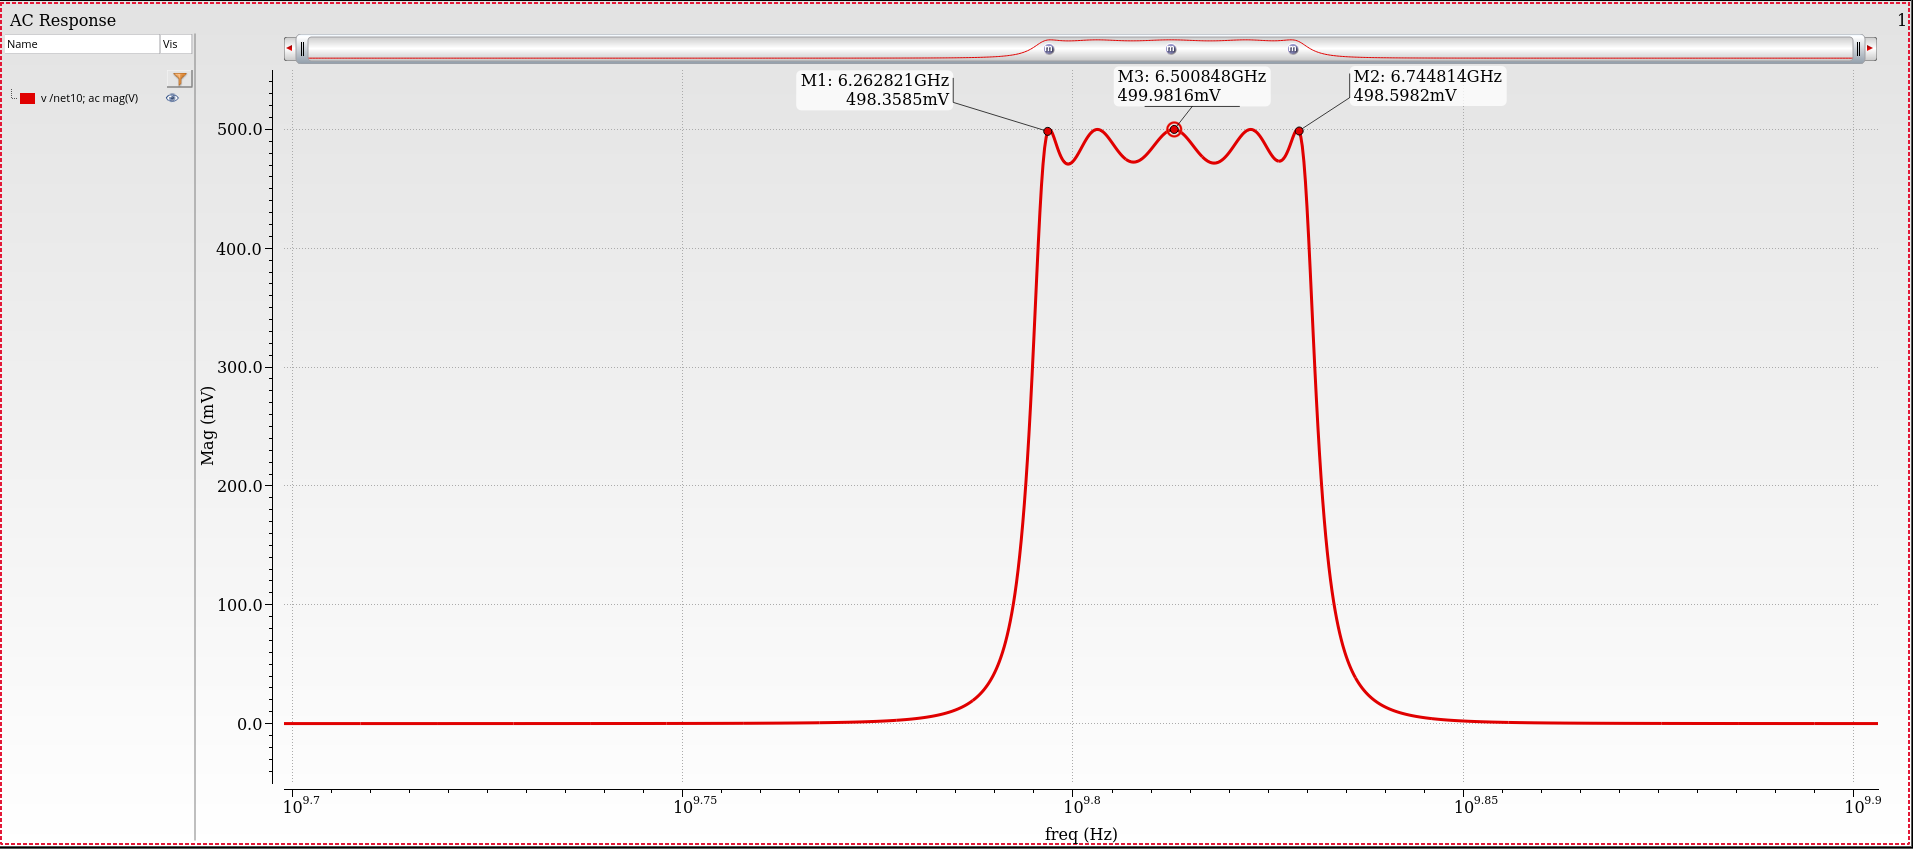
\includegraphics[width=0.95\linewidth]{Results/Fig/ac_mag_lin.png}
 \caption{Magnitude linear em $\text{mV}$ da resposta em frequência AC no nó \texttt{/net10}, que mostra os cinco ripples de Chebyshev na banda passante.}

    \label{fig:ac_mag_lin}
\end{figure}

Na curva em decibéis (Figura~\ref{fig:ac_mag_db}), o patamar máximo estabiliza em $-6{,}02\text{ dB}$ em $f_0 = 6{,}50\text{ GHz}$ devido ao divisor resistivo natural de $1/2$ ($20\log_{10}(0{,}5)$) formado pelas terminações de fonte e carga, apresentando ondulação interna limitada ao \textit{ripple} projetado de $0{,}5\text{ dB}$ (com mínimo de $-6{,}54\text{ dB}$ na borda inferior em $6{,}254\text{ GHz}$ e $-6{,}12\text{ dB}$ sobre a crista final em $6{,}748\text{ GHz}$, imediatamente antes da queda abrupta na borda superior de $6{,}75\text{ GHz}$, cujo mínimo teórico é $-6{,}52\text{ dB}$). Fora da banda passante, a atenuação acentua-se rapidamente, atingindo cerca de $25\text{ dB}$ de rejeição relativa nas bordas da especificação de largura total $1{,}5 \times BW$ ($6{,}125\text{ GHz}$ e $6{,}875\text{ GHz}$) e ultrapassando $40\text{ dB}$ em afastamentos de $\pm 500\text{ MHz}$ da portadora ($6{,}0\text{ GHz}$ e $7{,}0\text{ GHz}$), atendendo integralmente ao requisito mínimo de $25\text{ dB}$ do roteiro \cite{Filter1}.

\begin{figure}[!htbp]
    \centering
    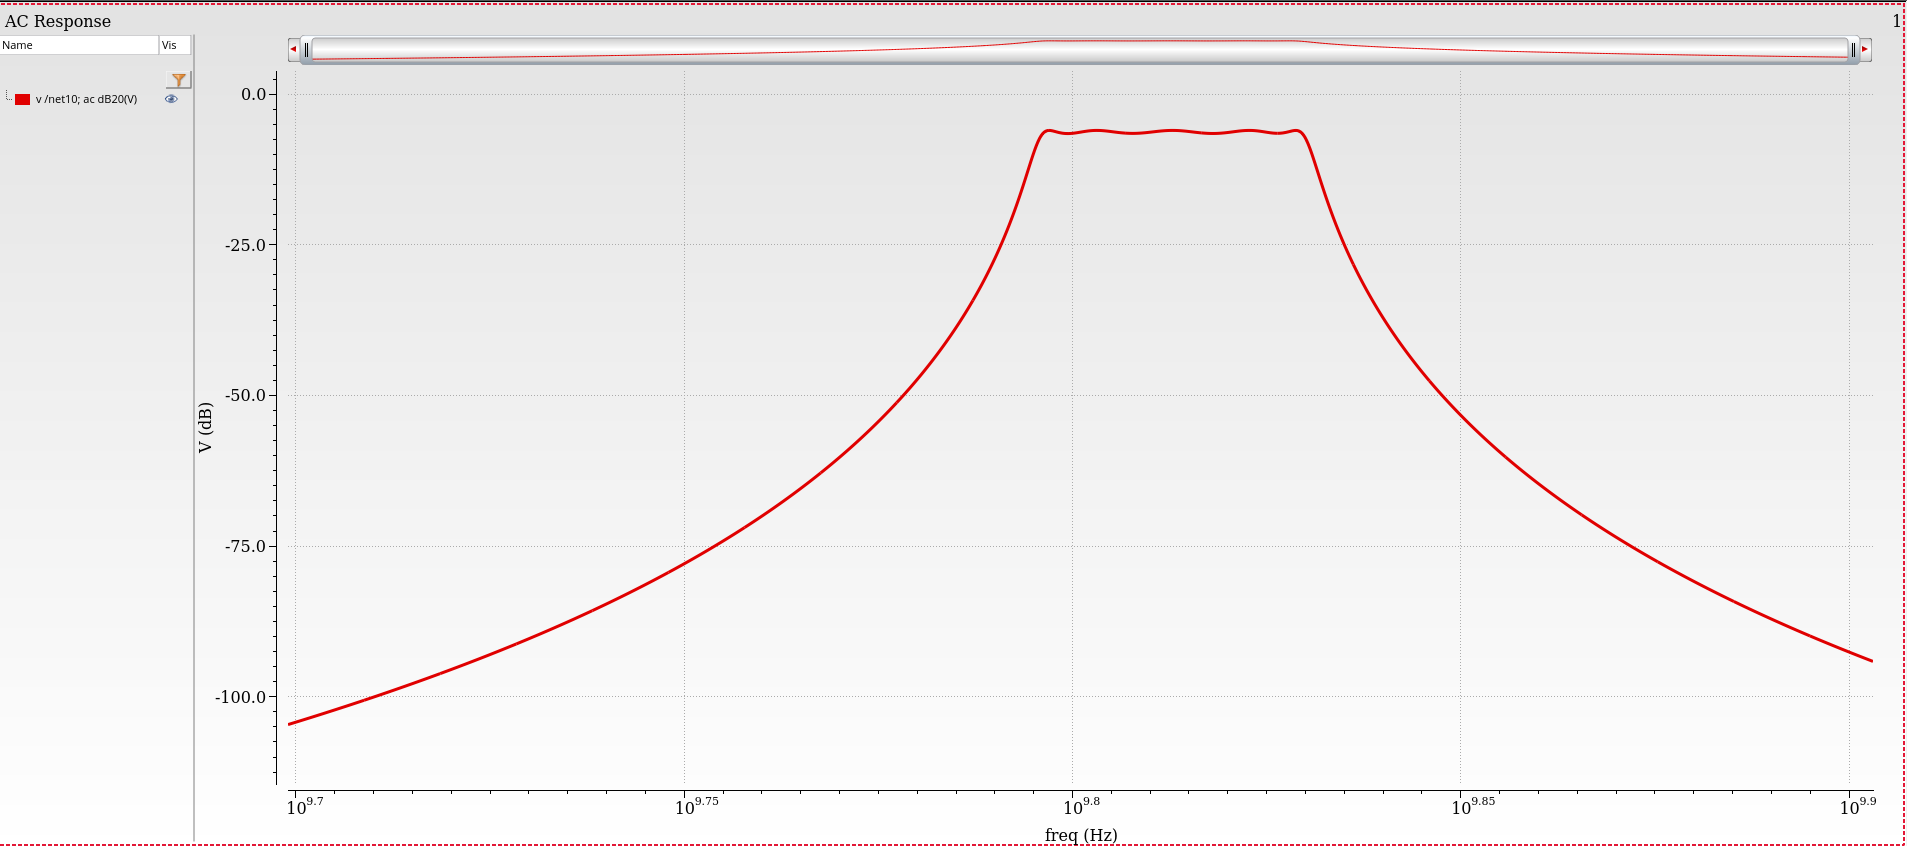
\includegraphics[width=0.95\linewidth]{Results/Fig/ac_mag_db.png}
    \caption{Magnitude em $\text{dB20}$ da resposta em frequência AC no nó \texttt{/net10}, destacando os marcadores de corte e o patamar de $-6{,}02\text{ dB}$.}
    \label{fig:ac_mag_db}
\end{figure}

A resposta de fase de $V_{\text{out}}$ (Figura~\ref{fig:ac_phase}) exibe comportamento monotônico e aproximadamente linear na região central da banda passante, cruzando $-363{,}88^\circ$ na frequência central de $6{,}504\text{ GHz}$. Ao longo da varredura de $5\text{ GHz}$ a $8\text{ GHz}$ (representada em eixo logarítmico, onde $10^{9{,}813}\text{ Hz} \approx 6{,}5\text{ GHz}$), observa-se uma excursão de fase de aproximadamente $872{,}6^\circ$ (de $+77{,}80^\circ$ em $5{,}255\text{ GHz}$ até $-794{,}85^\circ$ em $7{,}726\text{ GHz}$), tendendo assintoticamente aos $900^\circ$ ($10 \times 90^\circ$) esperados para os dez polos do sistema.

\begin{figure}[!htbp]
    \centering
    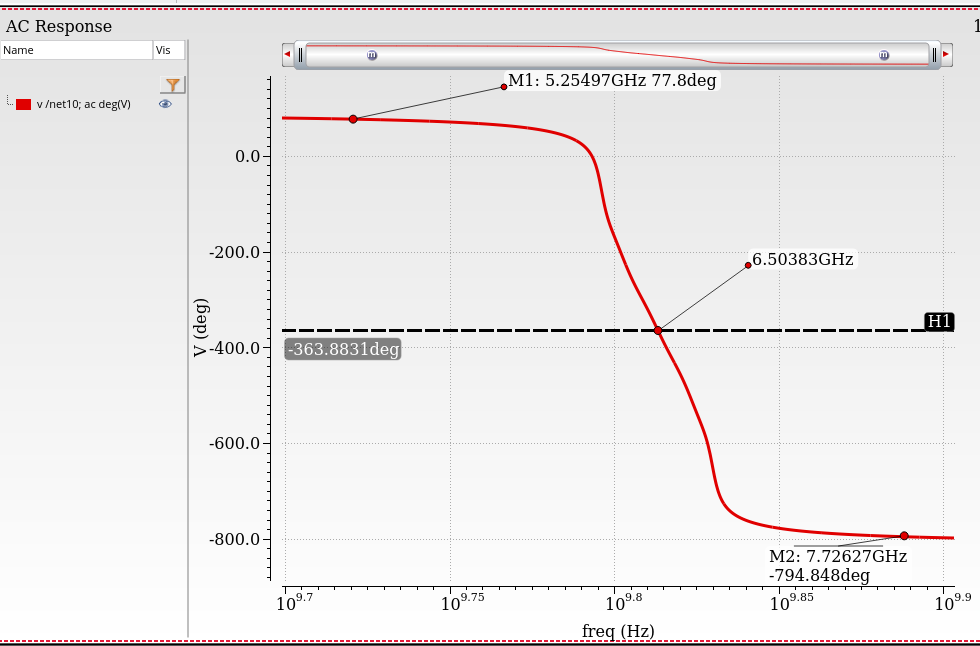
\includegraphics[width=0.95\linewidth]{Results/Fig/ac_phase.png}
    \caption{Resposta de fase em graus da tensão de saída \texttt{/net10} na simulação AC.}
    \label{fig:ac_phase}
\end{figure}

A distribuição de polos e zeros no plano complexo $s$ confirma a síntese analítica do filtro. Como esperado para uma transformação passa-faixa de quinta ordem, o circuito apresenta $10$ polos divididos em cinco pares complexos conjugados no semiplano esquerdo ($\text{Re}(s) < 0$, Figura~\ref{fig:pz_poles}), garantindo estabilidade incondicional. Os polos mais próximos do eixo imaginário situam-se nas bordas da banda passante ($6{,}252\text{ GHz}$ com $\sigma = -26{,}74\text{ MHz}$ e $6{,}757\text{ GHz}$ com $\sigma = -29{,}23\text{ MHz}$), sendo fisicamente responsáveis pela transição abrupta nas frequências de corte. Simultaneamente, o diagrama de zeros (Figura~\ref{fig:pz_zeros}) evidencia o zero na origem ($0\text{ Hz}$, de multiplicidade $N=5$ decorrente da transformação passa-faixa), assegurando o bloqueio completo de componentes DC.

\begin{figure}[!htbp]
    \centering
    \begin{minipage}[t]{0.48\linewidth}
        \centering
        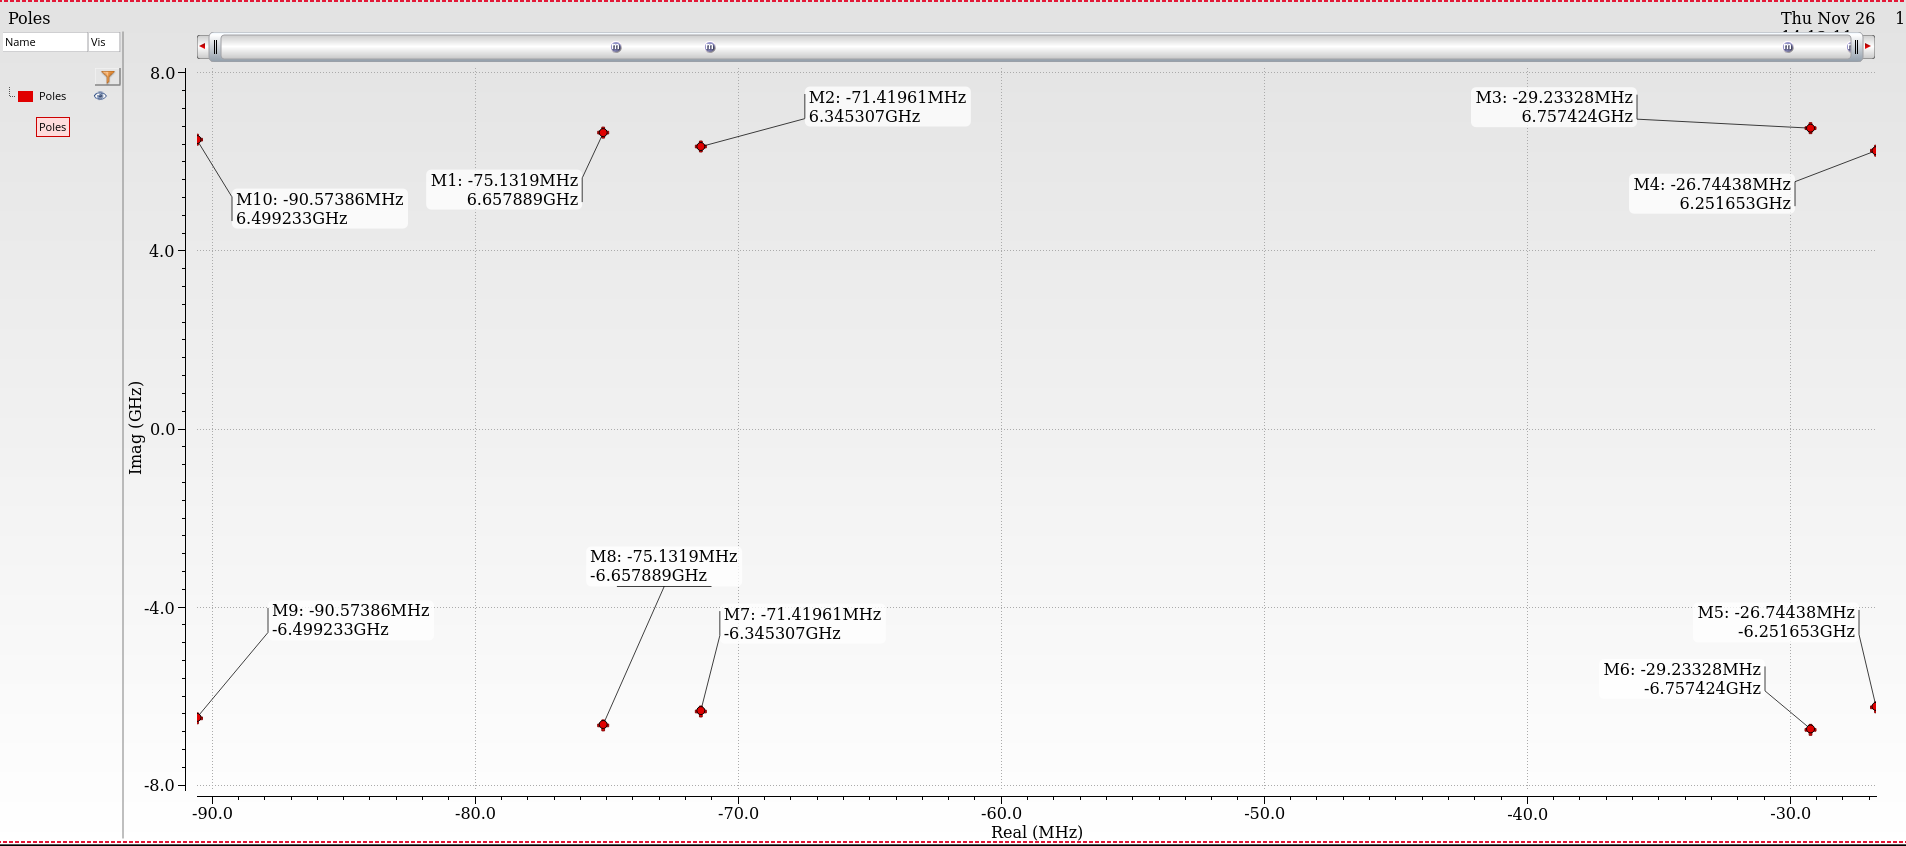
\includegraphics[width=\linewidth]{Results/Fig/pz_poles.png}
        \caption{Diagrama de polos no plano complexo $s$ ($6{,}25\text{ GHz}$ a $6{,}75\text{ GHz}$).}
        \label{fig:pz_poles}
    \end{minipage}
    \hfill
    \begin{minipage}[t]{0.48\linewidth}
        \centering
        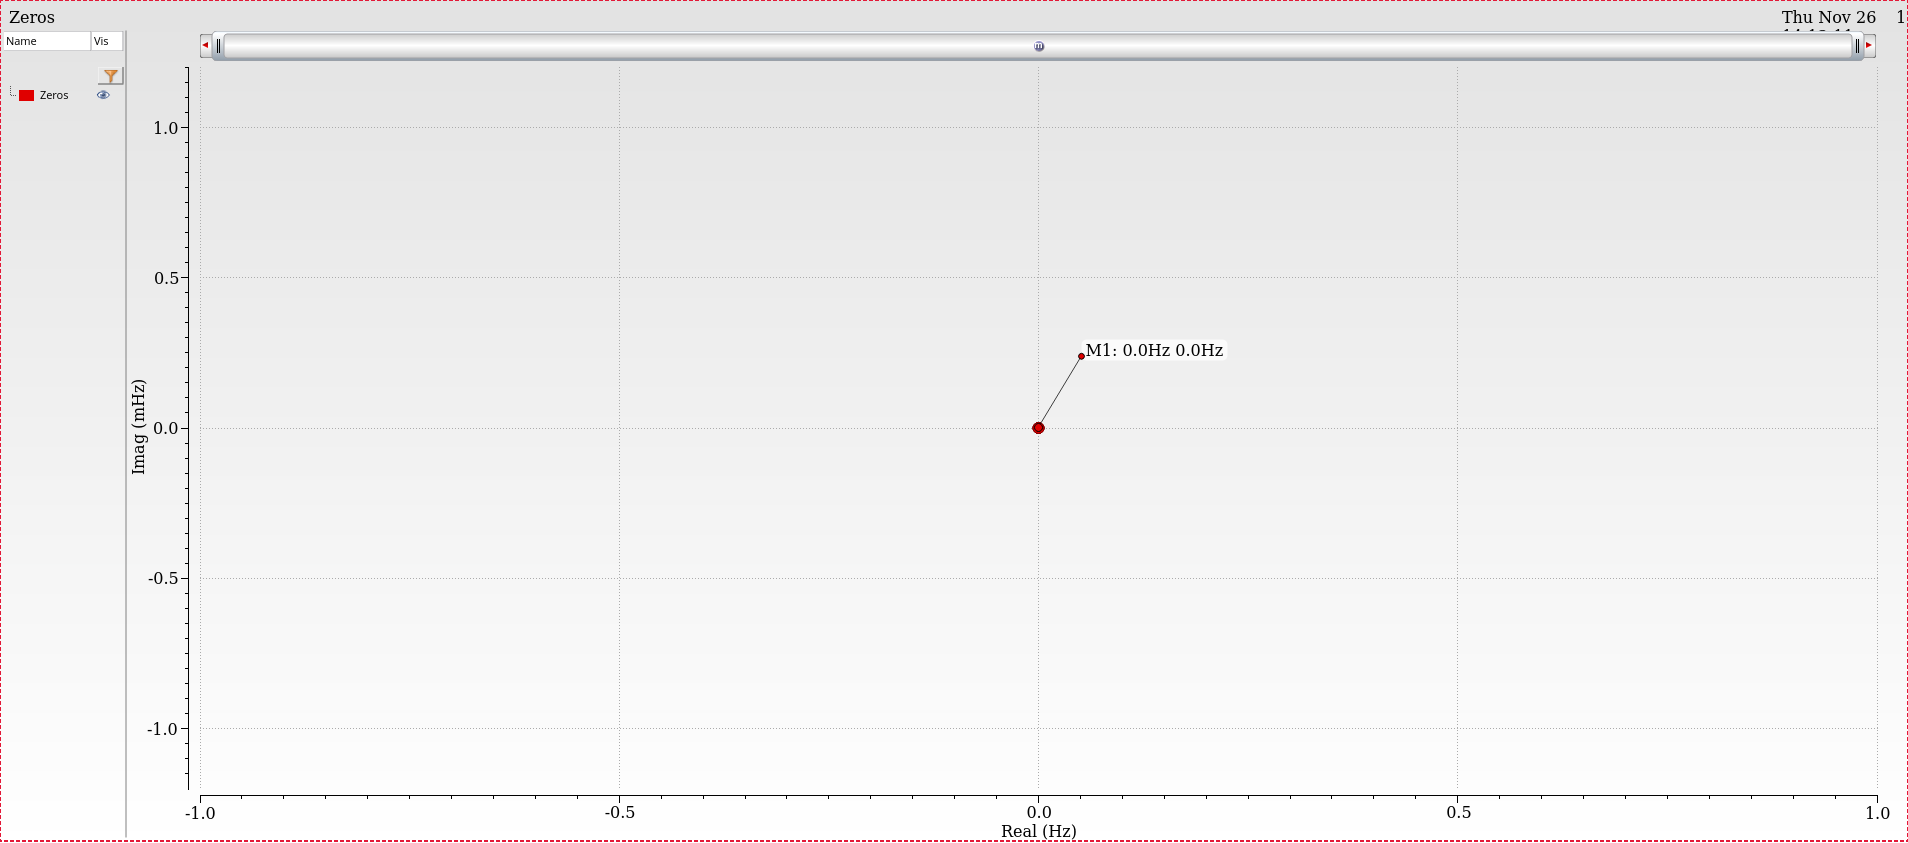
\includegraphics[width=\linewidth]{Results/Fig/pz_zeros.png}
        \caption{Diagrama de zeros no plano $s$ (multiplicidade $5$ na origem).}
        \label{fig:pz_zeros}
    \end{minipage}
\end{figure}

\subsection{Análise de Parâmetros de Espalhamento (SP)}

A caracterização de potência por parâmetros de espalhamento ratifica o desempenho de transmissão e casamento de impedância do filtro. Na resposta em banda larga de $5\text{ GHz}$ a $8\text{ GHz}$ (Figura~\ref{fig:sp_full}), a curva de transmissão direta $S_{21}$ atinge $0{,}00\text{ dB}$ ($-30{,}55~\mu\text{dB}$) na frequência central de $6{,}50\text{ GHz}$, confirmando perda de inserção (\textit{insertion loss}) nula para componentes ideais (variando até $0{,}50\text{ dB}$ nos vales do \textit{ripple} dentro da banda passante), enquanto a atenuação fora da banda alcança $-98{,}60\text{ dB}$ em $5{,}0\text{ GHz}$ e $-87{,}89\text{ dB}$ em $8{,}0\text{ GHz}$. Simultaneamente, devido à reciprocidade da rede passiva sem perdas, o coeficiente de transmissão reversa $S_{12}$ exibe comportamento idêntico a $S_{21}$.

\begin{figure}[!htbp]
    \centering
    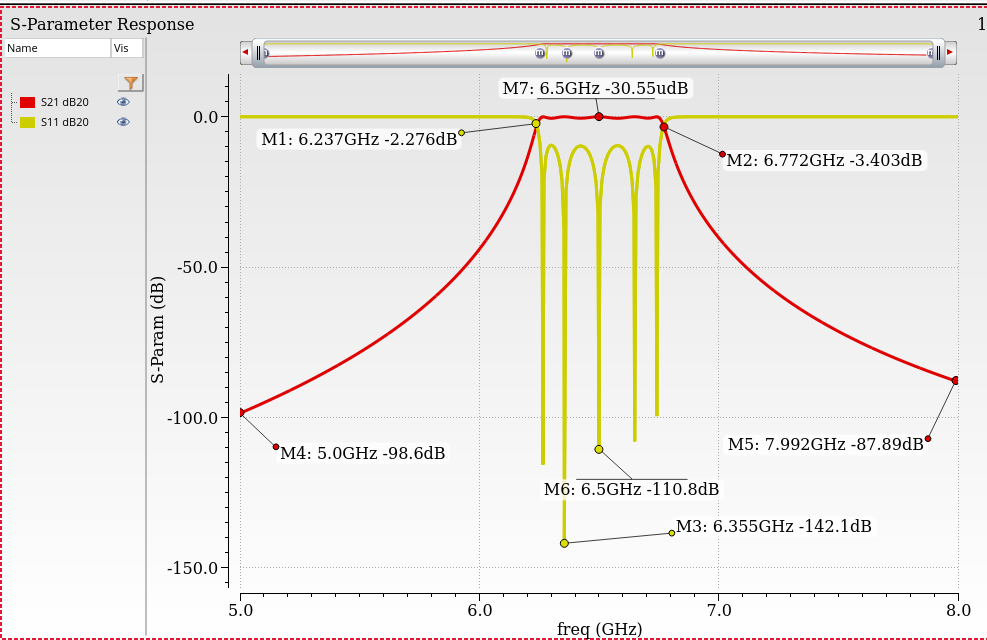
\includegraphics[width=0.95\linewidth]{Results/Fig/sp_s21_s11_full.png}
    \caption{Parâmetros de espalhamento $S_{21}$ e $S_{11}$ em $\text{dB20}$ de $5\text{ GHz}$ a $8\text{ GHz}$, evidenciando os cinco polos de reflexão na banda passante e a atenuação fora da banda.}
    \label{fig:sp_full}
\end{figure}

O coeficiente de reflexão na entrada ($S_{11}$) apresenta cinco vales profundos de casamento (atingindo $-142{,}15\text{ dB}$ em $6{,}355\text{ GHz}$ e $-110{,}84\text{ dB}$ em $6{,}50\text{ GHz}$), refletindo a simetria física da topologia também observada no coeficiente de reflexão de saída $S_{22}$ (Figura~\ref{fig:sp_s22}). Fora da banda passante, tanto $S_{11}$ quanto $S_{22}$ aproximam-se de $0\text{ dB}$, indicando que a potência dos sinais indesejados é refletida de volta à fonte em vez de ser dissipada internamente.

\begin{figure}[!htbp]
    \centering
    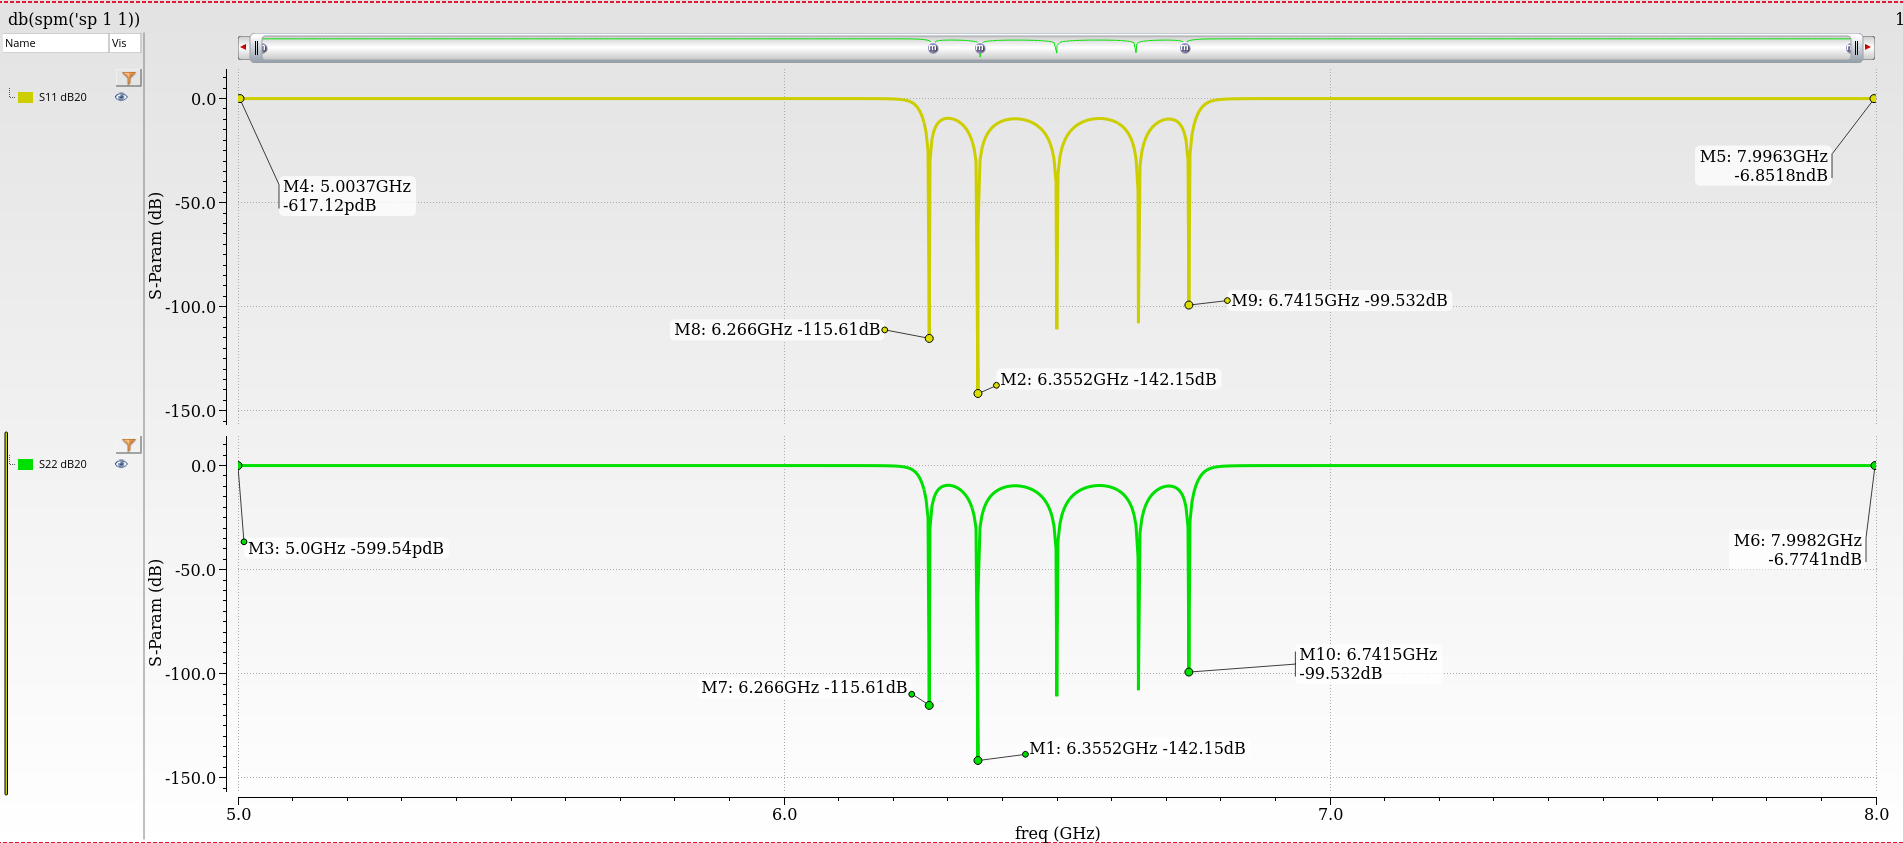
\includegraphics[width=0.95\linewidth]{Results/Fig/sp_s22.png}
    \caption{Coeficiente de reflexão na porta de saída ($S_{22}$) em $\text{dB20}$, comprovando a simetria da rede em relação a $S_{11}$.}
    \label{fig:sp_s22}
\end{figure}

No detalhamento da banda passante entre $6{,}0\text{ GHz}$ e $7{,}0\text{ GHz}$ (Figura~\ref{fig:sp_zoom}), observa-se que os arcos máximos de reflexão $S_{11}$ entre os vales de casamento limitam-se a aproximadamente $-9{,}64\text{ dB}$, valor teoricamente esperado para um \textit{ripple} de $0{,}5\text{ dB}$ ($|S_{11}|_{\max} = \sqrt{1 - 10^{-0{,}05}} \approx 0{,}3296$, equivalente a uma perda de retorno mínima de $9{,}64\text{ dB}$). Nos limites da faixa de rejeição especificada ($1{,}5 \times BW$ total), a transmissão direta $S_{21}$ atinge $-28{,}36\text{ dB}$ em $6{,}125\text{ GHz}$ e $-25{,}05\text{ dB}$ em $6{,}875\text{ GHz}$, cumprindo o critério mínimo de $25\text{ dB}$ de atenuação em ambos os lados da banda.

\begin{figure}[!htbp]
    \centering
    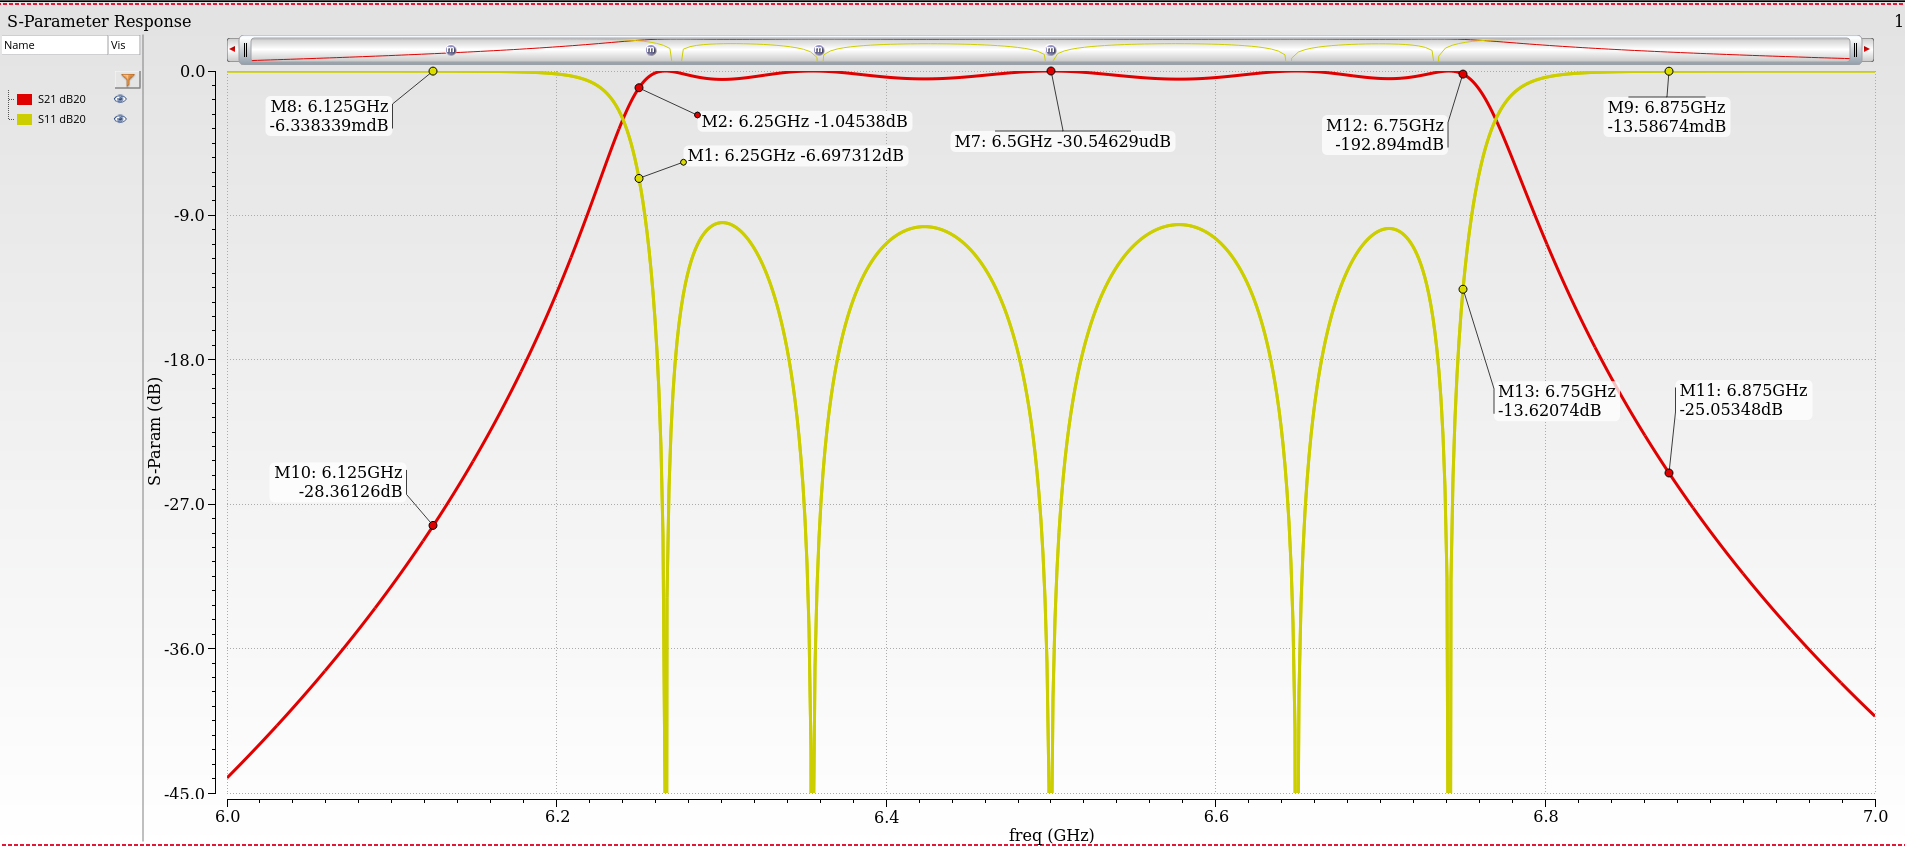
\includegraphics[width=0.95\linewidth]{Results/Fig/sp_zoom.png}
    \caption{Detalhe dos parâmetros $S_{21}$ e $S_{11}$ entre $6{,}0\text{ GHz}$ e $7{,}0\text{ GHz}$, destacando o \textit{ripple} na banda passante, o limite superior de $S_{11}$ ($\approx -9{,}64\text{ dB}$) e os pontos de atenuação em $6{,}125\text{ GHz}$ e $6{,}875\text{ GHz}$.}
    \label{fig:sp_zoom}
\end{figure}

A resposta de fase de $S_{21}$ (Figura~\ref{fig:sp_phase}) exibe variação monotônica e aproximadamente linear na região central da banda passante (cruzando $-360{,}19^\circ$ em $6{,}50\text{ GHz}$), característica desejável para minimizar a distorção de atraso de grupo ($\tau_g = -\mathrm{d}\phi/\mathrm{d}\omega$) no centro do canal, apresentando inclinação mais acentuada apenas próximo às frequências de corte. Entre $5{,}0\text{ GHz}$ e $8{,}0\text{ GHz}$, a fase varia de $+80{,}12^\circ$ até $-797{,}49^\circ$, perfazendo uma excursão total de $877{,}61^\circ$, coerente com a assíntota teórica de $900^\circ$ ($10 \times 90^\circ$) associada aos dez polos do filtro.

\begin{figure}[!htbp]
    \centering
    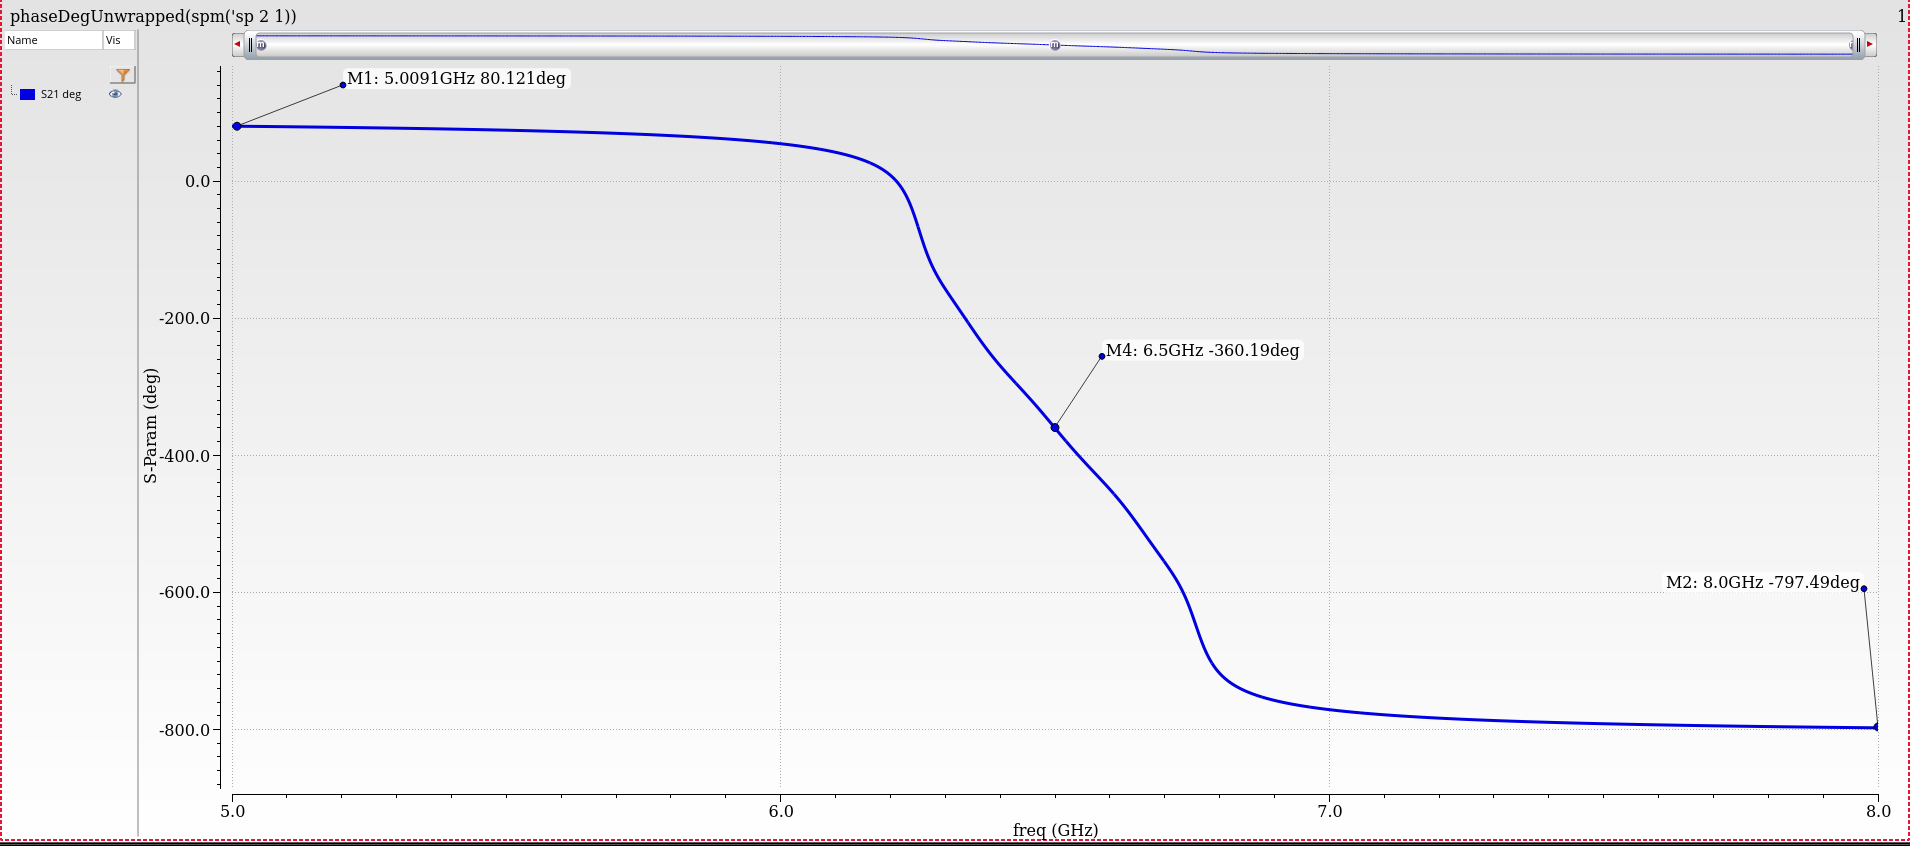
\includegraphics[width=0.95\linewidth]{Results/Fig/sp_phase.png}
    \caption{Resposta de fase do parâmetro $S_{21}$ em graus de $5\text{ GHz}$ a $8\text{ GHz}$.}
    \label{fig:sp_phase}
\end{figure}

A Tabela~\ref{tab:resumo_specs} consolida a comparação entre os requisitos de projeto e os valores medidos nas simulações lineares.

\begin{table}[!htbp]
\centering
\caption{Comparação entre as especificações do projeto e os resultados simulados (AC e SP).}
\label{tab:resumo_specs}
\setlength{\tabcolsep}{3pt}
\resizebox{\linewidth}{!}{%
\begin{tabular}{lccc}
\hline
\textbf{Parâmetro} & \textbf{Especificado} & \textbf{Simulado} & \textbf{Status} \\
\hline
Frequência central ($f_0$) & $6{,}50\text{ GHz}$ & $6{,}50\text{ GHz}$ & Atendido \\
Largura de banda ($BW$) & $500\text{ MHz}$ & $500\text{ MHz}$ & Atendido \\
Impedância terminal ($Z_0$) & $50~\Omega$ & $50~\Omega$ & Atendido \\
\textit{Ripple} na banda passante & $\le 1{,}0\text{ dB}$ & $0{,}50\text{ dB}$ & Atendido \\
Perda de inserção ($IL_{\min}$) & Ideal ($0\text{ dB}$) & $0{,}00\text{ dB}$ & Atendido \\
Perda de retorno mínima ($RL_{\min}$) & --- & \begin{tabular}[c]{@{}c@{}}$9{,}64\text{ dB}$\\($|S_{11}| \le -9{,}64\text{ dB}$)\end{tabular} & Coerente \\
Atenuação em $6{,}125 / 6{,}875\text{ GHz}$ ($1{,}5 \times BW$) & $\ge 25\text{ dB}$ & $28{,}36\text{ dB} / 25{,}05\text{ dB}$ & Atendido \\
Atenuação em $6{,}00 / 7{,}00\text{ GHz}$ ($f_0 \pm 500\text{ MHz}$) & $\ge 25\text{ dB}$ & $> 40\text{ dB}$ & Atendido \\
\hline
\end{tabular}%
}
\end{table}

\subsection{Avaliação Não Linear e Rejeição de Banda Adjacente (HB e Envelope)}

Para avaliar a rejeição a produtos de intermodulação e interferentes adjacentes gerados por não linearidades, analisou-se inicialmente o espectro multi-tom por balanço harmônico (\texttt{hb\_mt}) com a portadora útil em $f_1 = 6{,}5\text{ GHz}$ e um tom interferente em $f_2 = 6{,}0\text{ GHz}$ excitando o amplificador de potência (\texttt{PA\_PB}, ganho de $27{,}2\text{ dB}$ e $P_{1\text{dB}} = 5\text{ dBm}$). Conforme ilustrado na Figura~\ref{fig:hb_espectro} e quantificado na Tabela~\ref{tab:hb_mt}, a não linearidade cúbica do PA gera produtos de intermodulação de terceira ordem ($IM_3$) em $2f_1 - f_2 = 7{,}0\text{ GHz}$ e $2f_2 - f_1 = 5{,}5\text{ GHz}$. Na saída do filtro (\texttt{/net10}), a portadora útil em $6{,}5\text{ GHz}$ é preservada sem atenuação ($-6{,}38\text{ dBV}$ antes e após o filtro), enquanto o interferente em $6{,}0\text{ GHz}$ sofre rejeição de $49{,}66\text{ dB}$ e os produtos $IM_3$ em $7{,}0\text{ GHz}$ e $5{,}5\text{ GHz}$ são atenuados em $45{,}73\text{ dB}$ e $84{,}29\text{ dB}$, respectivamente.

\begin{figure}[!htbp]
    \centering
    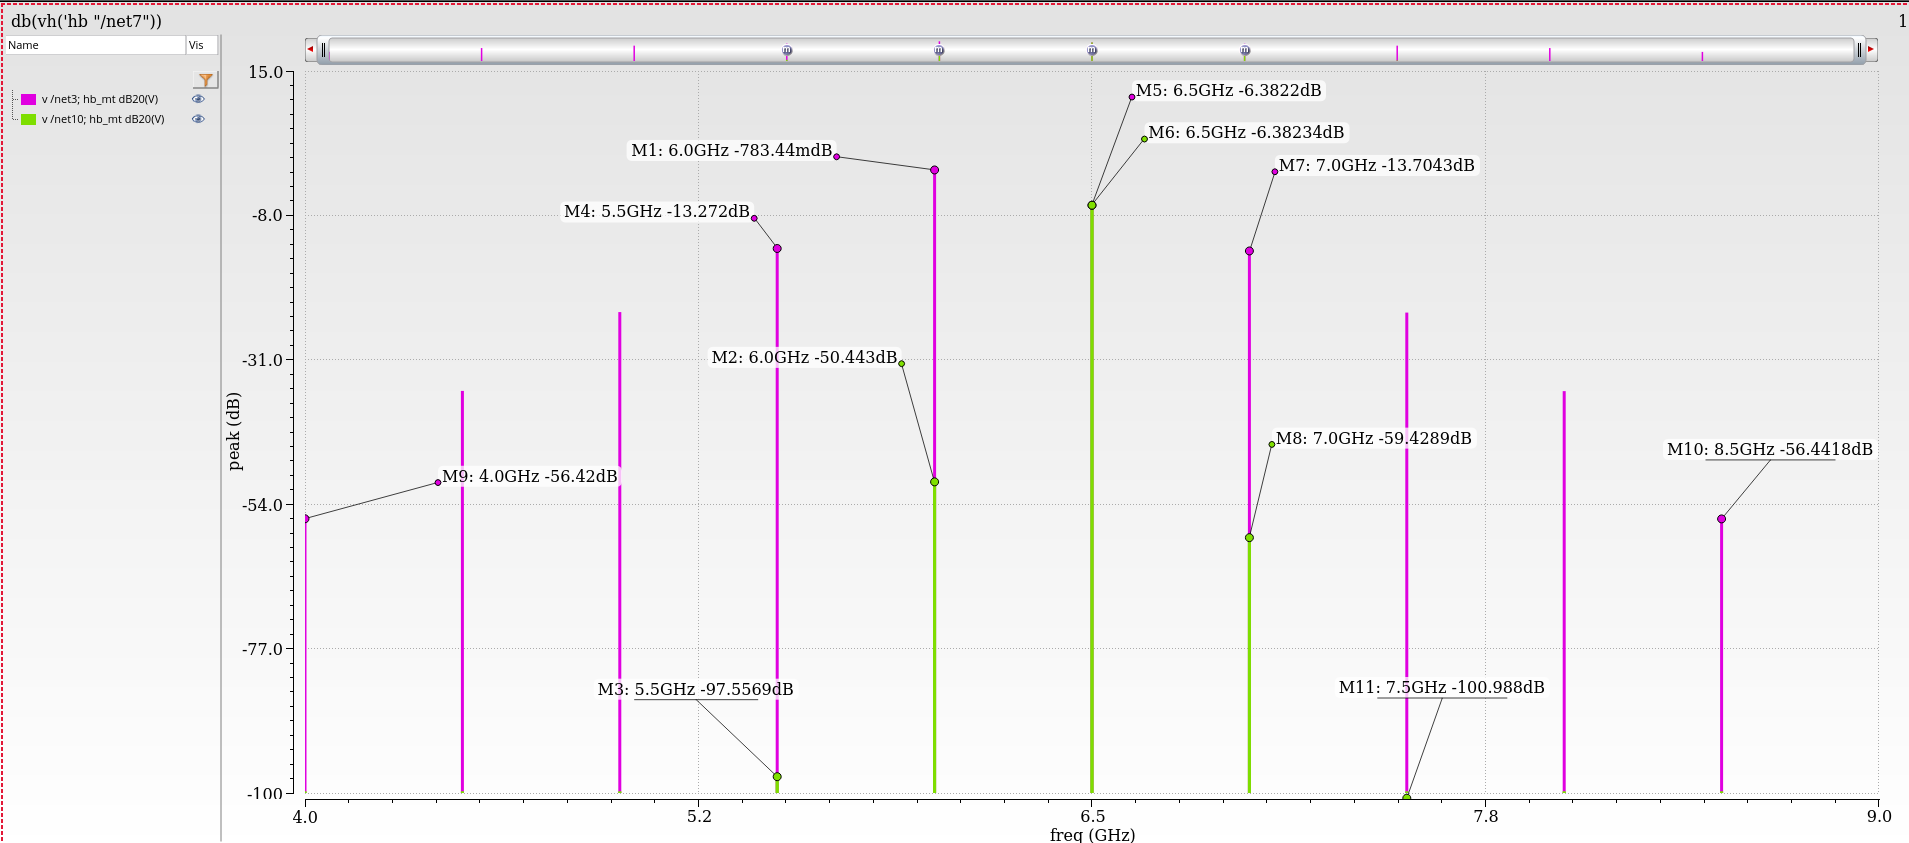
\includegraphics[width=\linewidth]{Results/Fig/hb_espectro.png}
    \caption{Espectro multi-tom (\texttt{hb\_mt}) na saída do PA (\texttt{/net3}, magenta) e após o filtro passa-faixa (\texttt{/net10}, verde), destacando a preservação do tom em $6{,}5\text{ GHz}$ e a supressão de $49{,}66\text{ dB}$ em $6{,}0\text{ GHz}$.}
    \label{fig:hb_espectro}
\end{figure}

\begin{table}[!htbp]
    \centering
    \caption{Níveis de tensão espectral antes e após o filtro na análise multi-tom (\texttt{hb\_mt}).}
    \label{tab:hb_mt}
    \resizebox{\linewidth}{!}{%
    \begin{tabular}{lccc}
        \hline
        \textbf{Componente Espectral} & \textbf{Pós-PA (\texttt{/net3})} & \textbf{Pós-Filtro (\texttt{/net10})} & \textbf{Rejeição (dB)} \\
        \hline
        Portadora útil ($6{,}5\text{ GHz}$) & $-6{,}38\text{ dBV}$ & $-6{,}38\text{ dBV}$ & $0{,}00\text{ dB}$ \\
        Interferente adjacente ($6{,}0\text{ GHz}$) & $-0{,}78\text{ dBV}$ & $-50{,}44\text{ dBV}$ & $49{,}66\text{ dB}$ \\
        Produto $IM_3$ superior ($7{,}0\text{ GHz}$) & $-13{,}70\text{ dBV}$ & $-59{,}43\text{ dBV}$ & $45{,}73\text{ dB}$ \\
        Produto $IM_3$ inferior ($5{,}5\text{ GHz}$) & $-13{,}27\text{ dBV}$ & $-97{,}56\text{ dBV}$ & $84{,}29\text{ dB}$ \\
        \hline
    \end{tabular}%
    }
\end{table}

Na sequência, realizou-se a análise de envelope (\texttt{envlp}) com o sinal modulado OFDM 16-QAM em $6{,}5\text{ GHz}$ (Figura~\ref{fig:psdacpr}). O sinal de entrada (\texttt{WPRB0}) apresenta potência média de $-0{,}04\text{ dBm}$ ($-36{,}61\text{ mdBm}$) e razão de potência no canal adjacente (ACPR) de $-65{,}79\text{ dBc}$ (inferior) e $-65{,}73\text{ dBc}$ (superior). Ao atravessar o amplificador de potência operando próximo à região de compressão ($P_{\text{in}} = 0\text{ dBm}$, $P_{1\text{dB}} = 5\text{ dBm}$), a potência média no canal eleva-se para $5{,}42\text{ dBm}$ (\texttt{WPRB1}) e o alargamento espectral (\textit{spectral regrowth}) degrada o ACPR em $\pm 40\text{ MHz}$ para $-19{,}69\text{ dBc}$ e $-19{,}71\text{ dBc}$. Na saída do filtro (\texttt{WPRB2}), o ACPR medido em $\pm 40\text{ MHz}$ permanece em $-18{,}56\text{ dBc}$ e $-18{,}54\text{ dBc}$, pois esse afastamento situa-se integralmente dentro da banda passante de $500\text{ MHz}$ ($\pm 250\text{ MHz}$ em torno de $6{,}5\text{ GHz}$), enquanto a rejeição atua sobre produtos de intermodulação e interferentes afastados ($\ge 375\text{ MHz}$ da portadora). A pequena diferença de $+0{,}13\text{ dB}$ na potência média integrada em \texttt{WPRB2} ($5{,}55\text{ dBm}$) decorre da integração numérica da PSD na janela da sonda aliada ao descasamento reativo entre a saída do PA e a impedância do filtro fora da banda.

\begin{figure}[!htbp]
    \centering
    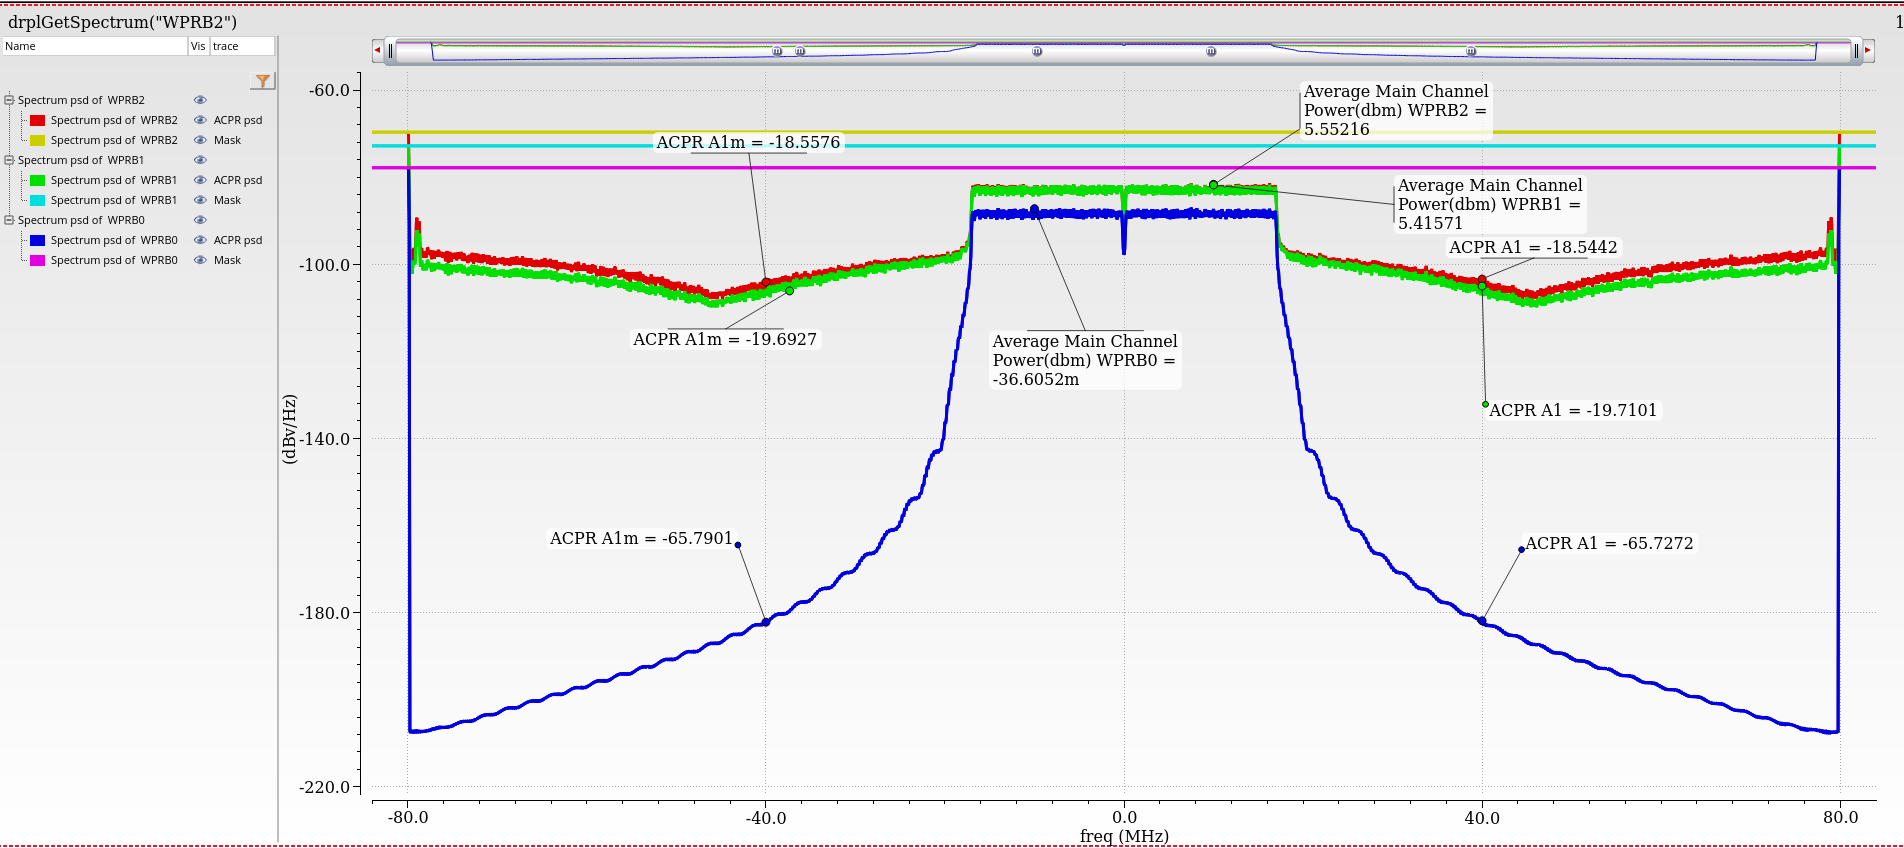
\includegraphics[width=\linewidth]{Results/Fig/PSD e ACPR.png}
    \caption{Densidade Espectral de Potência (PSD) e Razão de Potência no Canal Adjacente (ACPR) nas sondas \texttt{WPRB0}, \texttt{WPRB1} e \texttt{WPRB2}.}
    \label{fig:psdacpr}
\end{figure}

No domínio da potência, confirma-se a compressão dos picos de envoltória responsável pelo espalhamento espectral, conforme ilustrado pelas curvas de CCDF na Figura~\ref{fig:CCDF}. O sinal OFDM original (\texttt{WPRB0}) exibe relação pico-média (PAPR) de até $10{,}92\text{ dB}$, valor que é reduzido para $7{,}84\text{ dB}$ após o ceifamento no amplificador (\texttt{WPRB1}) e para $3{,}11\text{ dB}$ na saída do filtro (\texttt{WPRB2}), refletindo o corte das componentes espectrais de alta frequência responsáveis pelos transientes rápidos de envoltória.

\begin{figure}[!htbp]
    \centering
    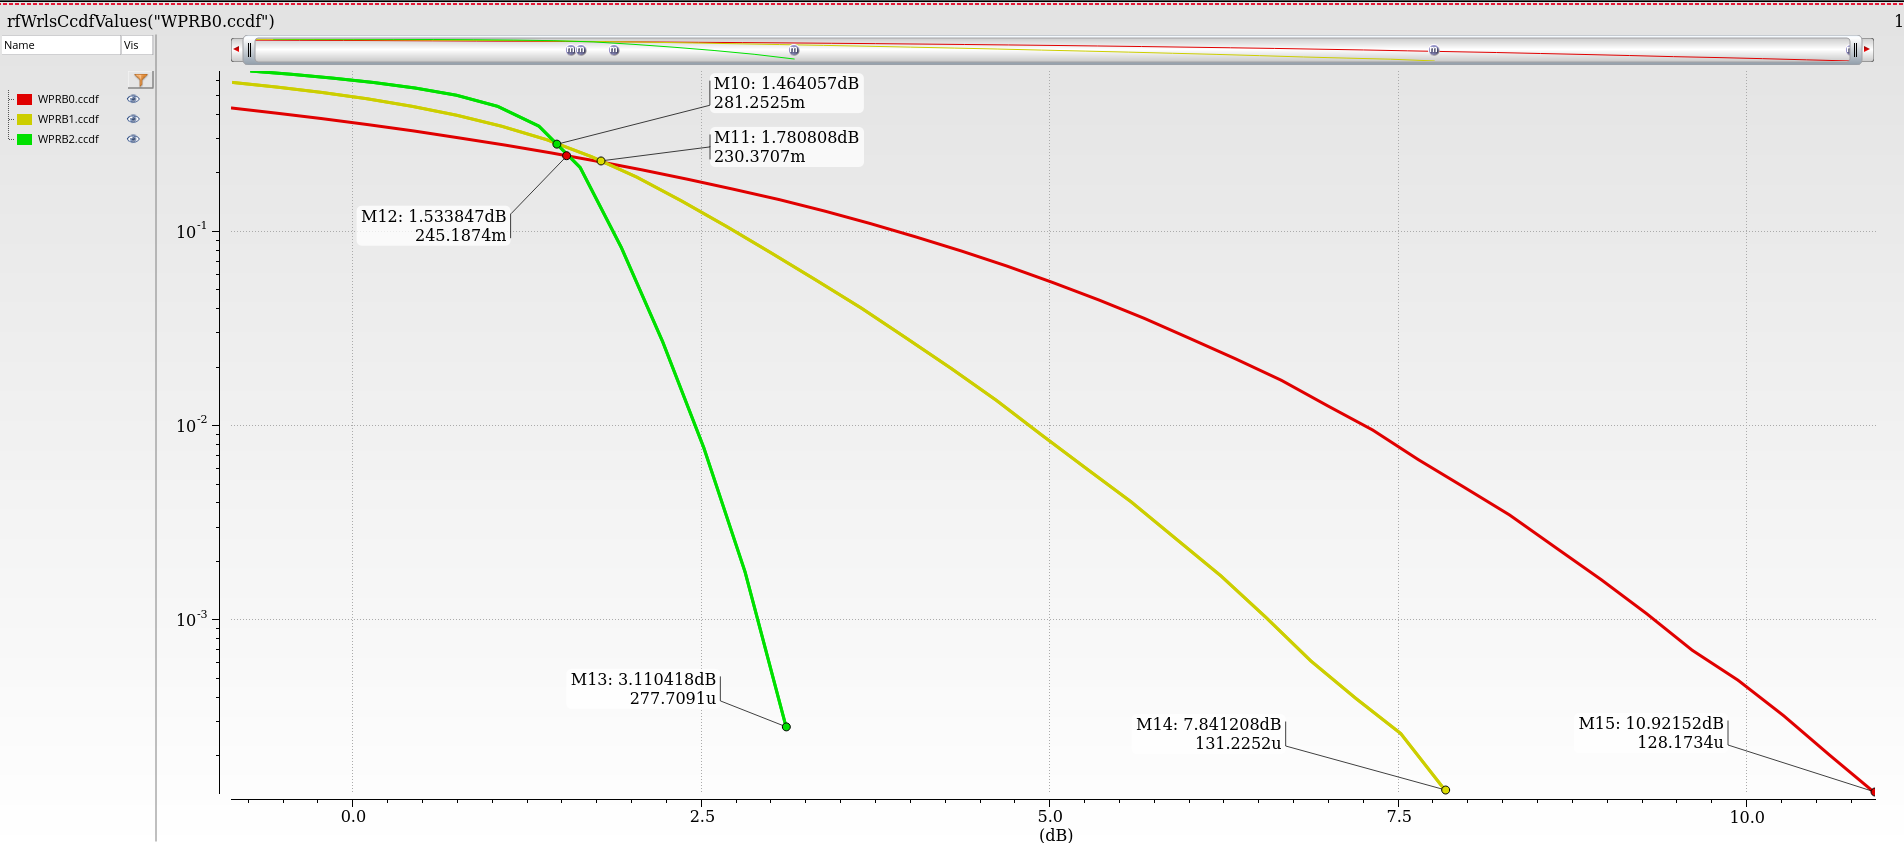
\includegraphics[width=\linewidth]{Results/Fig/CCDF.png}
    \caption{Função de Distribuição Cumulativa Complementar (CCDF) do sinal nas sondas \texttt{WPRB0}, \texttt{WPRB1} e \texttt{WPRB2}.}
    \label{fig:CCDF}
\end{figure}

No domínio da modulação, a comparação entre o sinal gerado pela fonte e o sinal distorcido após o amplificador está representada nas Figuras~\ref{fig:const_wprb0} e~\ref{fig:const_wprb1}, enquanto a Tabela~\ref{tab:nonlinear} consolida todas as métricas extraídas nas três sondas. Na entrada (\texttt{WPRB0}), os $16$ símbolos apresentam erro residual desprezível ($\mathrm{EVM} = 0{,}03\%$ e $\mathrm{BER} = 0\%$). Após a saturação do amplificador (\texttt{WPRB1}), as distorções não lineares de amplitude e fase (AM-AM e AM-PM) dispersam os símbolos da constelação, elevando o $\mathrm{EVM}$ para $28{,}10\%$ e a $\mathrm{BER}$ para $4{,}88\%$. Na saída do filtro (\texttt{WPRB2}), a atenuação de componentes espúrias fora da banda reduz parcialmente o erro para $\mathrm{EVM} = 23{,}74\%$ e $\mathrm{BER} = 2{,}58\%$, demonstrando fisicamente que o filtro suprime interferências e harmônicas externas, mas não corrige distorções geradas dentro da própria banda passante.

\begin{figure}[!htbp]
    \centering
    \begin{subfigure}[b]{0.8\linewidth}
        \centering
        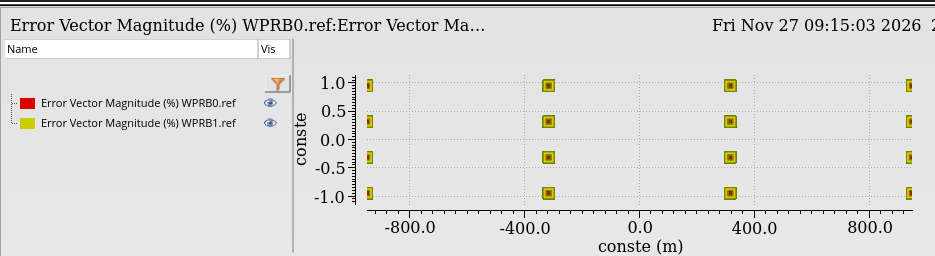
\includegraphics[width=\linewidth]{Results/Fig/Constelação 16-QAM 3.png}
        \caption{Saída da fonte (\texttt{WPRB0}, $\text{EVM} = 0{,}03\%$).}
        \label{fig:const_wprb0}
    \end{subfigure}
    
    \vspace{0.4cm}
    
    \begin{subfigure}[b]{0.8\linewidth}
        \centering
        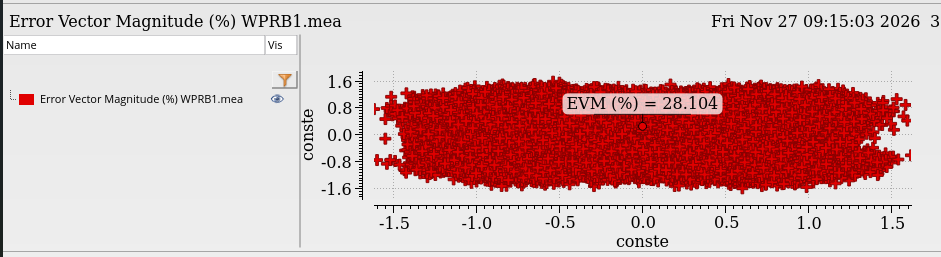
\includegraphics[width=\linewidth]{Results/Fig/Constelação 16-QAM 2.png}
        \caption{Pós-PA (\texttt{WPRB1}, $\text{EVM} = 28{,}10\%$).}
        \label{fig:const_wprb1}
    \end{subfigure}
    \caption{Constelações 16-QAM e medidas de EVM.}
    \label{fig:constelacoes_qam}
\end{figure}


\begin{table}[!htbp]
    \centering
    \caption{Resumo das métricas não lineares e de modulação obtidas na simulação de envelope.}
    \label{tab:nonlinear}
    \resizebox{\linewidth}{!}{%
    \begin{tabular}{lccc}
        \hline
        \textbf{Métrica} & \textbf{WPRB0 (Fonte)} & \textbf{WPRB1 (Pós-PA)} & \textbf{WPRB2 (Pós-Filtro)} \\
        \hline
        Potência Média no Canal & $-0{,}04\text{ dBm}$ & $5{,}42\text{ dBm}$ & $5{,}55\text{ dBm}$ \\
        ACPR Inferior / Superior & $-65{,}79 / -65{,}73\text{ dBc}$ & $-19{,}69 / -19{,}71\text{ dBc}$ & $-18{,}56 / -18{,}54\text{ dBc}$ \\
        PAPR Máximo (CCDF) & $10{,}92\text{ dB}$ & $7{,}84\text{ dB}$ & $3{,}11\text{ dB}$ \\
        Taxa de Erro de Bit (BER) & $0\%$ & $4{,}88\%$ & $2{,}58\%$ \\
        EVM (\%) & $0{,}03\%$ & $28{,}10\%$ & $23{,}74\%$ \\
        \hline
    \end{tabular}%
    }
\end{table}
%\section{Amplificadores de Múltiplos Estágios (Lab 1)}


\subsection{Questão 1 -- Amplificador Fonte-Comum com Transistor NMOS}

\subsubsection{Item 1.a -- Esquemático e Dimensionamento dos Elementos Passivos}

\paragraph{Metodologia}
\vspace{0.2cm}
Conforme especificado no roteiro~\cite{AMP2_1}, propôs-se a topologia de amplificador fonte-comum ilustrada na Figura~\ref{fig:esquematico_nmos}, sendo sua respectiva implementação modelada no ambiente Cadence Virtuoso conforme mostrado na Figura~\ref{fig:esquematico1}. Todas as simulações foram conduzidas no simulador Cadence Spectre (processo TSMC $65\text{ nm}$ CMOS) à temperatura de $40^\circ\text{C}$, com os arquivos de esquemático e simulação organizados no diretório \texttt{\textasciitilde/cadence/tsmc65/Amp2/Lab1} (\texttt{schematic} e \texttt{maestro}).

O transistor \texttt{nmos\_rf} foi dimensionado com largura total $W = 30\ \mu\text{m}$ distribuída em $15$ \textit{fingers} ($2\ \mu\text{m}$ por \textit{finger}) e comprimento de canal igual a quatro vezes o mínimo da tecnologia ($L = 4 \times 60\text{ nm} = 240\text{ nm}$). Na etapa inicial, aplicou-se uma fonte senoidal de entrada de frequência $f = 2\text{ MHz}$ com amplitude de $1\text{ mV}$, resistência de fonte $R_{Sig} = 50\ \Omega$, alimentação $V_{DD} = 1.2\text{ V}$, polarização $V_{Bias}$ e carga $R_L = 2\text{ k}\Omega$. Para determinar os valores mínimos e nominais adequados dos elementos passivos de acoplamento ($C_{in}$, $C_{out}$) e polarização ($L_{in}$, $L_{out}$), realizou-se o cálculo analítico em Python considerando os critérios de reatância na frequência de operação ($X_C = \frac{1}{2\pi f C} \ll R$ para curtos-circuitos AC e $X_L = 2\pi f L \gg R$ para circuitos abertos AC).

\begin{figure}[H]
    \centering
\begin{circuitikz}[american, thick]
    % Estilo para os terminais de alimentação (barra horizontal)
    \tikzset{vrail/.style={draw, line width=1.2pt}}

    % Transistor NMOS principal
    \draw (0,0) node[nmos] (M1) {};
    % Terra do Source
    \draw (M1.S) -- (0,-1.5) node[tground] {};

    % Indutor de dreno e alimentação V_DD
    \draw (M1.D) -- (0,1.2) to[L] (0,2.8) -- (0,3.2);
    \draw[vrail] (-0.4,3.2) -- (0.4,3.2) node[midway, above] {$\mathrm{V_{DD}}$};

    % Ramo da esquerda (Gate, Bias, v_in, C_in, R_Sig, v_Sig)
    \draw (M1.G) -- (-1.5,0) coordinate (N_bias);
    
    % Indutor de polarização e V_Bias
    \draw (N_bias) to[L] (-1.5,2.2) -- (-1.5,2.6);
    \draw[vrail] (-1.9,2.6) -- (-1.1,2.6) node[midway, above] {$\mathrm{V_{Bias}}$};

    % Nó v_in
    \draw (N_bias) -- (-2.5,0) coordinate (N_vin);
    \draw (N_vin) -- (-2.5,0.6) node[ocirc] {} node[above, blue] {$\mathcal{V}_{in}$};

    % Capacitor de acoplamento de entrada
    \draw (N_vin) to[C] (-3.8,0) coordinate (N_cin);

    % Parte em cinza da entrada (R_Sig e v_Sig)
    \begin{scope}[color=black]
        \draw (N_cin) to[R, l_=$\mathcal{R}_{Sig}$] (-5.3,0)
              to[V, v=$\mathcal{V}_{Sig}$] (-5.3,-1.5) node[tground] {};
    \end{scope}

    % Ramo da direita (Dreno, C_out, R_L, v_out)
    \draw (M1.D) -- (0,1.0) coordinate (N_drain);
    \draw (N_drain) to[C] (2.2,1.0) coordinate (N_cout);

    % Parte em cinza da saída (R_L)
    \begin{scope}[color=black]
        \draw (N_cout) to[R, l=$\mathcal{R}_{L}$] (2.2,-0.8) node[tground] {};
    \end{scope}

    % Nó v_out
    \draw (N_cout) -- (3.2,1.0) node[ocirc] {} node[above, blue] {$\mathcal{V}_{out}$};

\end{circuitikz}
    \caption{Esquemático do amplificador fonte-comum com transistor NMOS.}
    \label{fig:esquematico_nmos}
\end{figure}

\begin{figure}[H]
    \centering
    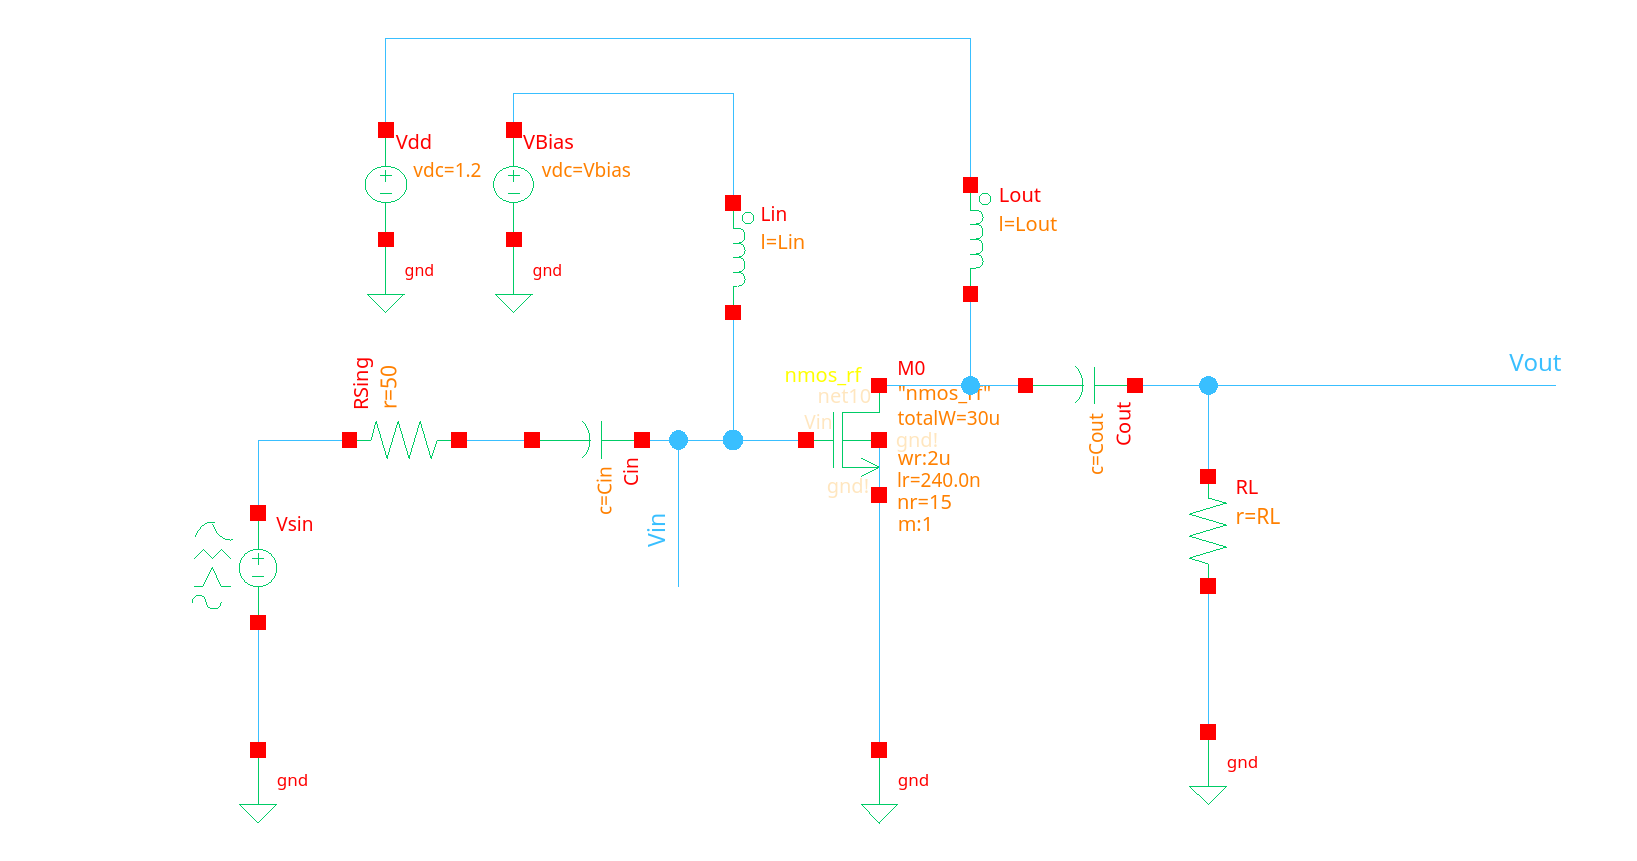
\includegraphics[width=0.82\textwidth]{Geral/Fig/Esquematico 1.png}
    \caption{Esquemático do amplificador fonte-comum com transistor NMOS, modelado no Cadence.}
    \label{fig:esquematico1}
\end{figure}

\paragraph{Resultados}
\vspace{0.2cm}
A Tabela~\ref{tab:passivos} sintetiza os valores mínimos obtidos via cálculo em Python para a frequência de $2\text{ MHz}$, juntamente com os valores nominais adotados no esquemático do Cadence para garantir o regime ideal de pequenos sinais.

\begin{table}[H]
    \centering
    \caption{Dimensionamento dos componentes passivos para $f = 2\text{ MHz}$.}
    \label{tab:passivos}
    \begin{tabular}{lcc}
        \hline
        \textbf{Componente} & \textbf{Mínimo Calculado} & \textbf{Valor Adotado} \\
        \hline
        $C_{in}$ & $15.92\text{ nF}$ & $1\ \mu\text{F}$ \\
        $C_{out}$ & $3.98\text{ nF}$ & $1\ \mu\text{F}$ \\
        $L_{in}$ & $0.40\text{ mH}$ & $10\text{ mH}$ \\
        $L_{out}$ (com $R_L = 2\text{ k}\Omega$) & $15.92\text{ mH}$ & $100\text{ mH}$ \\
        $L_{out}$ (circuito aberto) & $99.47\text{ mH}$ & $100\text{ mH}$ \\
        \hline
    \end{tabular}
\end{table}

\paragraph{Conclusão}
\vspace{0.2cm}
A adoção de capacitores de $1\ \mu\text{F}$ ($X_C \approx 79.6\ \text{m}\Omega$) e indutores de $10\text{ mH}$ ($X_{Lin} \approx 125.7\ \text{k}\Omega$) e $100\text{ mH}$ ($X_{Lout} \approx 1.257\ \text{M}\Omega$) isola completamente os pontos de polarização DC dos sinais AC de $2\text{ MHz}$, eliminando divisores capacitivos e desvios de corrente AC tanto na condição com carga quanto em circuito aberto.

\subsubsection{Item 1.b -- Simulação Transiente e Ganho de Tensão}

\paragraph{Metodologia}
\vspace{0.2cm}
Após a conclusão do esquemático, criou-se a vista \texttt{maestro} (teste \texttt{Amp2\_Lab1}), na qual foi executada uma análise transiente (\texttt{tran}) no ponto de polarização em saturação ($V_{Bias} \approx 780\text{ mV}$) com carga $R_L = 2\text{ k}\Omega$. Para eliminar a influência do transitório inicial de carga dos elementos reativos ($C$ e $L$), o ganho de tensão de pequenos sinais foi avaliado em regime permanente na janela de $2\ \mu\text{s}$ a $5\ \mu\text{s}$ ($6$ ciclos completos do sinal de $f = 2\text{ MHz}$, cujo período é $T = 1/f = 0.5\ \mu\text{s}$) por meio da expressão \texttt{Ganho\_Av} configurada na tabela de saídas (\textit{Outputs Setup}) do ADE Explorer (onde \texttt{/net1} corresponde ao nó de saída \texttt{/Vout}):
\begin{equation}
    |A_v| = \frac{\text{peakToPeak}(\text{clip}(V_T(\text{''/net1''}), 2\mu, 5\mu))}{\text{peakToPeak}(\text{clip}(V_T(\text{''/Vin''}), 2\mu, 5\mu))}
\end{equation}
Adicionalmente, configurou-se a razão instantânea ponto a ponto entre os sinais totais de saída e entrada para verificar o comportamento temporal do estágio:
\begin{equation}
    A_{v,\text{inst}}(t) = \frac{V_T(\text{''/net1''})}{V_T(\text{''/Vin''})}
\end{equation}

\paragraph{Resultados}
\vspace{0.2cm}
Analiticamente, na frequência de $2\text{ MHz}$, os capacitores atuam como curtos-circuitos e os indutores como circuitos abertos ($v_{gs} = v_{in}$). Aplicando a Lei das Correntes de Kirchhoff (LCK) no nó de dreno, obtém-se a expressão algébrica do ganho de tensão de pequenos sinais:
\begin{equation}
    A_v = \frac{v_{out}}{v_{in}} = -g_m \cdot (r_o \parallel R_L) = -g_m \cdot \left(\frac{r_o \cdot R_L}{r_o + R_L}\right)
\end{equation}

Substituindo a resistência de carga $R_L = 2\text{ k}\Omega$ e os parâmetros intrínsecos de pequenos sinais do transistor \texttt{nmos\_rf} no ponto de polarização ($g_m = 8.42\text{ mS}$ e $r_o = 25\text{ k}\Omega$ no dimensionamento analítico, ou $g_m = 10.42\text{ mS}$ e $r_o = 5.761\text{ k}\Omega$ extraídos via \texttt{OP("/M0")}), obtém-se o ganho teórico assintótico entre $15.47\text{ V/V}$ e $15.59\text{ V/V}$:
\begin{equation}
    |A_{v,\text{teórico}}| = 8.42\text{ mS} \times \left(\frac{25\text{ k}\Omega \times 2\text{ k}\Omega}{25\text{ k}\Omega + 2\text{ k}\Omega}\right) = 15.59\text{ V/V}
\end{equation}

Para provar que os resultados apresentados nos gráficos do Cadence ViVA estão matematicamente corretos, confrontaram-se as equações teóricas com as leituras diretas das formas de onda:
\begin{enumerate}
    \item \textbf{Validação do Gráfico Transiente (Figura~\ref{fig:transiente_vout_vin}):} Com uma excitação senoidal de entrada de amplitude $1.0\text{ mV}$ ($\Delta V_{in,\text{pp}} = 2.0\text{ mV}$) e período $T = 500.0\text{ ns}$ ($f = 2.0\text{ MHz}$), a saída apresenta excursão pico a pico de $\Delta V_{out,\text{pp}} = 30.98\text{ mV}$ (amplitude de $15.49\text{ mV}$). A razão direta entre essas amplitudes fornece:
    \begin{equation}
        |A_{v,\text{gráfico}}| = \frac{\Delta V_{out,\text{pp}}}{\Delta V_{in,\text{pp}}} = \frac{30.98\text{ mV}}{2.0\text{ mV}} = 15.49\text{ V/V}
    \end{equation}
    Esse valor coincide exatamente com a leitura automatizada \texttt{Ganho\_Av = 15.49} exibida no gráfico e apresenta desvio de apenas $0.64\%$ em relação ao ganho teórico assintótico ($15.59\text{ V/V}$), validando a expressão da Calculator.

    \item \textbf{Validação da Razão Instantânea e Inversão de Fase (Figura~\ref{fig:av_inst}):} Como a expressão \texttt{Av\_Inst} divide o sinal total de saída $V_{out}(t)$ (nível DC nulo devido a $C_{out}$) pelo sinal total de entrada $V_{in}(t) = V_{DC} + v_{in}(t)$ (onde $V_{DC} \approx 780\text{ mV}$ e $v_{in,\text{pico}} = 1\text{ mV}$), e sendo o estágio fonte-comum \textbf{inversor} ($180^\circ$ de defasagem), os extremos teóricos da curva devem ocorrer nos picos opostos de $V_{in}$ e $V_{out}$:
    \begin{equation}
        A_{v,\text{inst(máx)}} = \frac{+15.40\text{ mV}}{780\text{ mV} - 1\text{ mV}} = +19.77\text{ m} \qquad \text{e} \qquad A_{v,\text{inst(mín)}} = \frac{-15.34\text{ mV}}{780\text{ mV} + 1\text{ mV}} = -19.64\text{ m}
    \end{equation}
    Esses valores teóricos coincidem exatamente com os marcadores medidos no gráfico da Figura~\ref{fig:av_inst} (\texttt{M1 = 19.7699m} e \texttt{M2 = -19.6366m}, com período $T = 499.8\text{ ns}$), comprovando matematicamente tanto a inversão de fase do amplificador quanto a exatidão numérica de ambas as curvas simuladas.
\end{enumerate}

\begin{figure}[H]
    \centering
    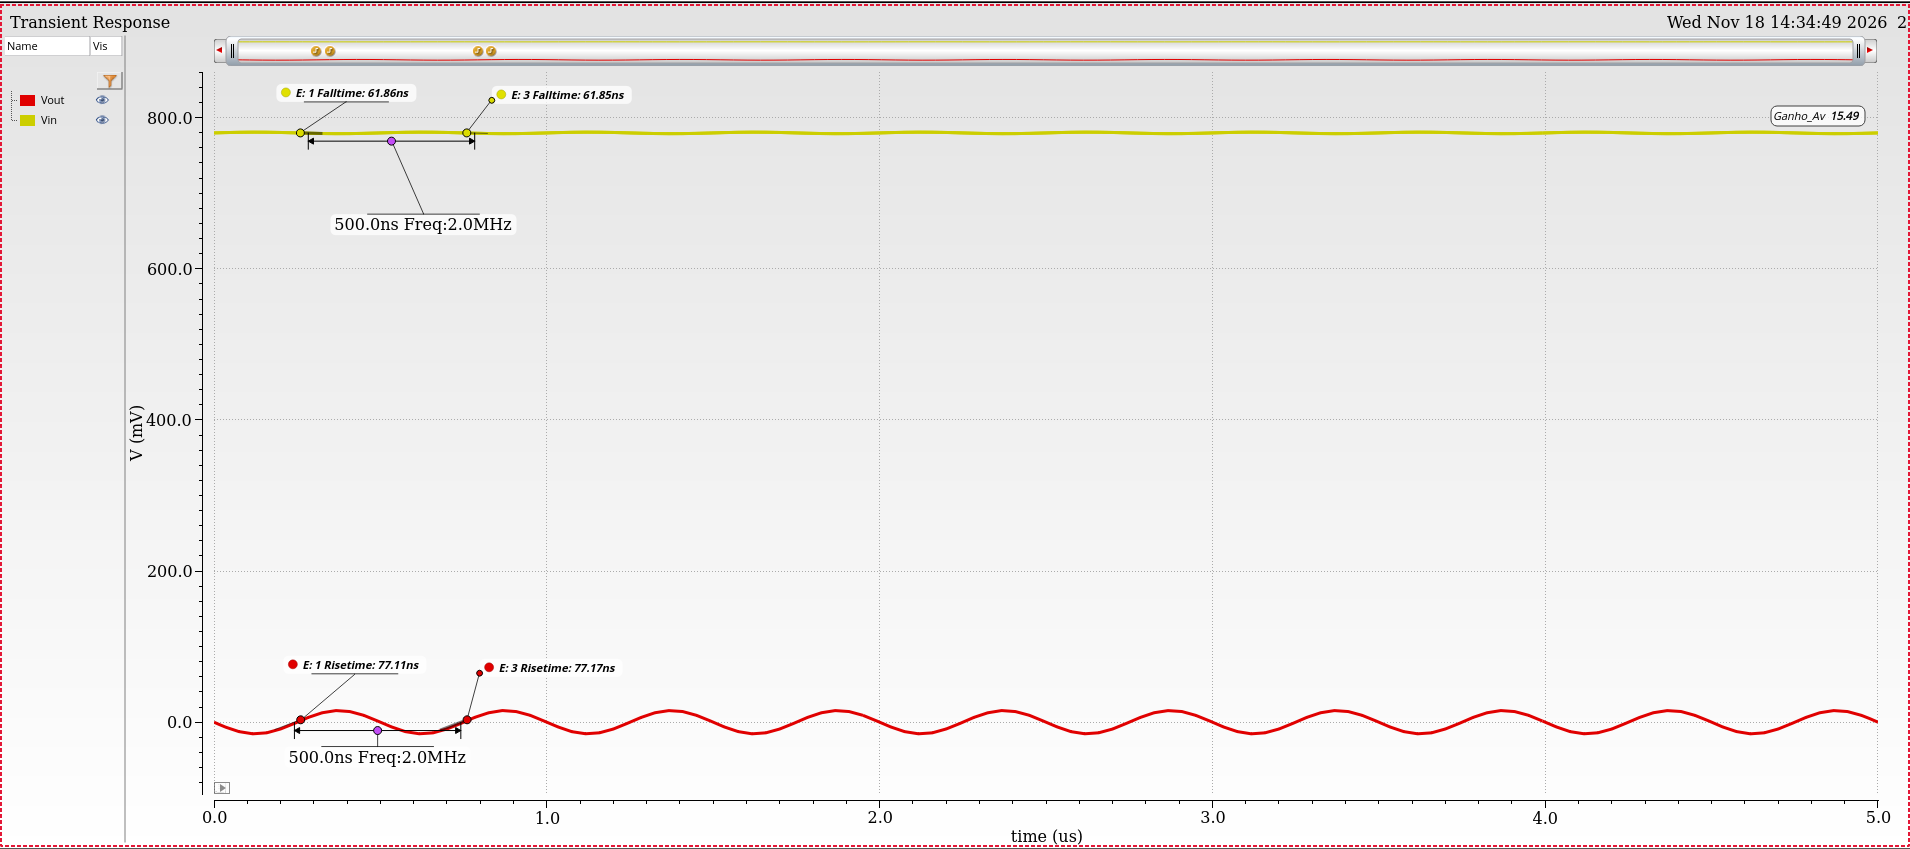
\includegraphics[width=0.92\textwidth]{Geral/Fig/transiente_vout_vin.png}
    \caption{Formas de onda transientes de $V_{in}$ e $V_{out}$ em $f = 2.0\text{ MHz}$ ($T = 500\text{ ns}$) e valor calculado de $|A_v| = 15.49\text{ V/V}$.}
    \label{fig:transiente_vout_vin}
\end{figure}

\begin{figure}[H]
    \centering
    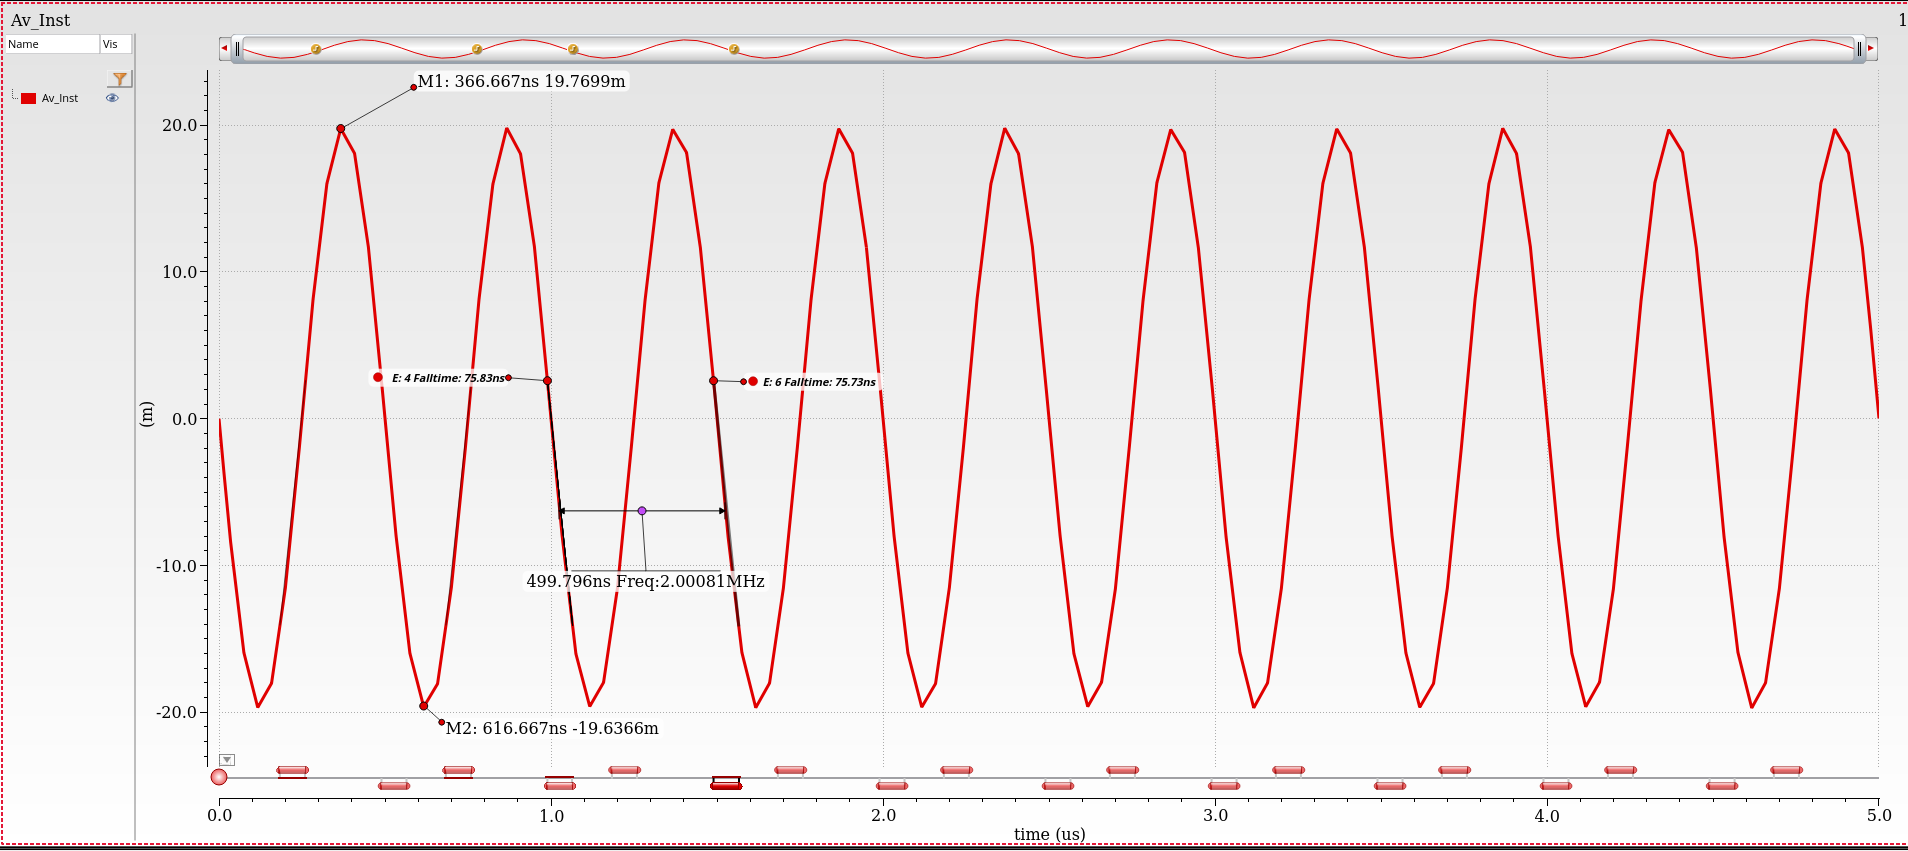
\includegraphics[width=0.92\textwidth]{Geral/Fig/av_inst.png}
    \caption{Forma de onda da razão instantânea \texttt{Av\_Inst} ($V_T(\text{''/Vout''})/V_T(\text{''/Vin''})$), evidenciando o período de $499.8\text{ ns}$ ($f \approx 2.0\text{ MHz}$) e os marcadores \texttt{M1 = 19.77m} e \texttt{M2 = -19.64m}.}
    \label{fig:av_inst}
\end{figure}

\paragraph{Conclusão}
\vspace{0.2cm}
A comprovação numérica entre as equações analíticas e as leituras diretas dos marcadores nos gráficos confirma que o estágio fonte-comum opera linearmente na saturação com ganho inversor de $|A_v| = 15.49\text{ V/V}$ (erro de $0.64\%$ frente ao modelo teórico assintótico). Além disso, a demonstração matemática dos picos de \texttt{Av\_Inst} ($+19.77\text{ m}$ e $-19.64\text{ m}$) prova que a expressão automatizada \texttt{Ganho\_Av} com a função \texttt{peakToPeak} está correta e é indispensável para isolar a excursão AC do nível DC de polarização nas análises subsequentes.

\subsubsection{Item 1.c -- Determinação do Ganho em Circuito Aberto ($A_{vo} \approx 60$)}

\paragraph{Metodologia}
\vspace{0.2cm}
Removeu-se a carga externa ($R_L \to \infty$) para avaliar o ganho de tensão intrínseco em circuito aberto ($A_{vo} = -g_m \cdot r_o$). Na tabela de saídas do ADE Explorer, definiu-se a expressão \texttt{Ganho\_Av} na janela estabilizada de $2\ \mu\text{s}$ a $5\ \mu\text{s}$ (além da razão instantânea \texttt{Av\_Inst = VT("/Vout") / VT("/Vin")}):
\begin{equation}
    |A_{vo}| = \frac{\text{peakToPeak}(\text{clip}(V_T(\text{''/Vout''}), 2\mu, 5\mu))}{\text{peakToPeak}(\text{clip}(V_T(\text{''/Vin''}), 2\mu, 5\mu))}
\end{equation}
Para determinar o valor de $V_{Bias}$ ($0 < V_{Bias} \le V_{DD}$) que resulta em $|A_{vo}| \approx 60\text{ V/V}$, realizou-se primeiramente uma varredura paramétrica ampla de $0\text{ mV}$ a $1200\text{ mV}$ com passo linear de $100\text{ mV}$, seguida de uma inspeção detalhada nas regiões de cruzamento e de uma varredura fina com passo de $0.5\text{ mV}$ na faixa de operação estável.

\paragraph{Resultados}
\vspace{0.2cm}
Na varredura ampla (Figura~\ref{fig:varredura_geral}), observou-se que a curva cruza o patamar de $60\text{ V/V}$ em duas regiões distintas: uma na faixa inferior, em torno de $V_{Bias} = 278.27\text{ mV}$ (situada entre $200\text{ mV}$, com ganho de $10.7\text{ V/V}$, e $300\text{ mV}$, com ganho de $73.68\text{ V/V}$), e outra na faixa superior, entre $700\text{ mV}$ (com ganho de $64.41\text{ V/V}$) e $800\text{ mV}$ (com ganho de $58.65\text{ V/V}$). Ao analisar detalhadamente a região inferior entre $200\text{ mV}$ e $300\text{ mV}$ (Figura~\ref{fig:varredura_inferior}), verificaram-se múltiplos cruzamentos instáveis ($274.27\text{ mV}$, $291.61\text{ mV}$ e $295.97\text{ mV}$) decorrentes da operação do transistor em corte/inversão fraca ($V_{GS} < V_{th}$). Na varredura fina entre $700\text{ mV}$ e $800\text{ mV}$ com passo de $0.5\text{ mV}$ (Figura~\ref{fig:varredura_fina}), identificou-se o cruzamento exato em $V_{Bias} = 779.8\text{ mV}$ (próximo ao valor interpolado de $776.54\text{ mV}$) para $|A_{vo}| = 60\text{ V/V}$.

\begin{figure}[H]
    \centering
    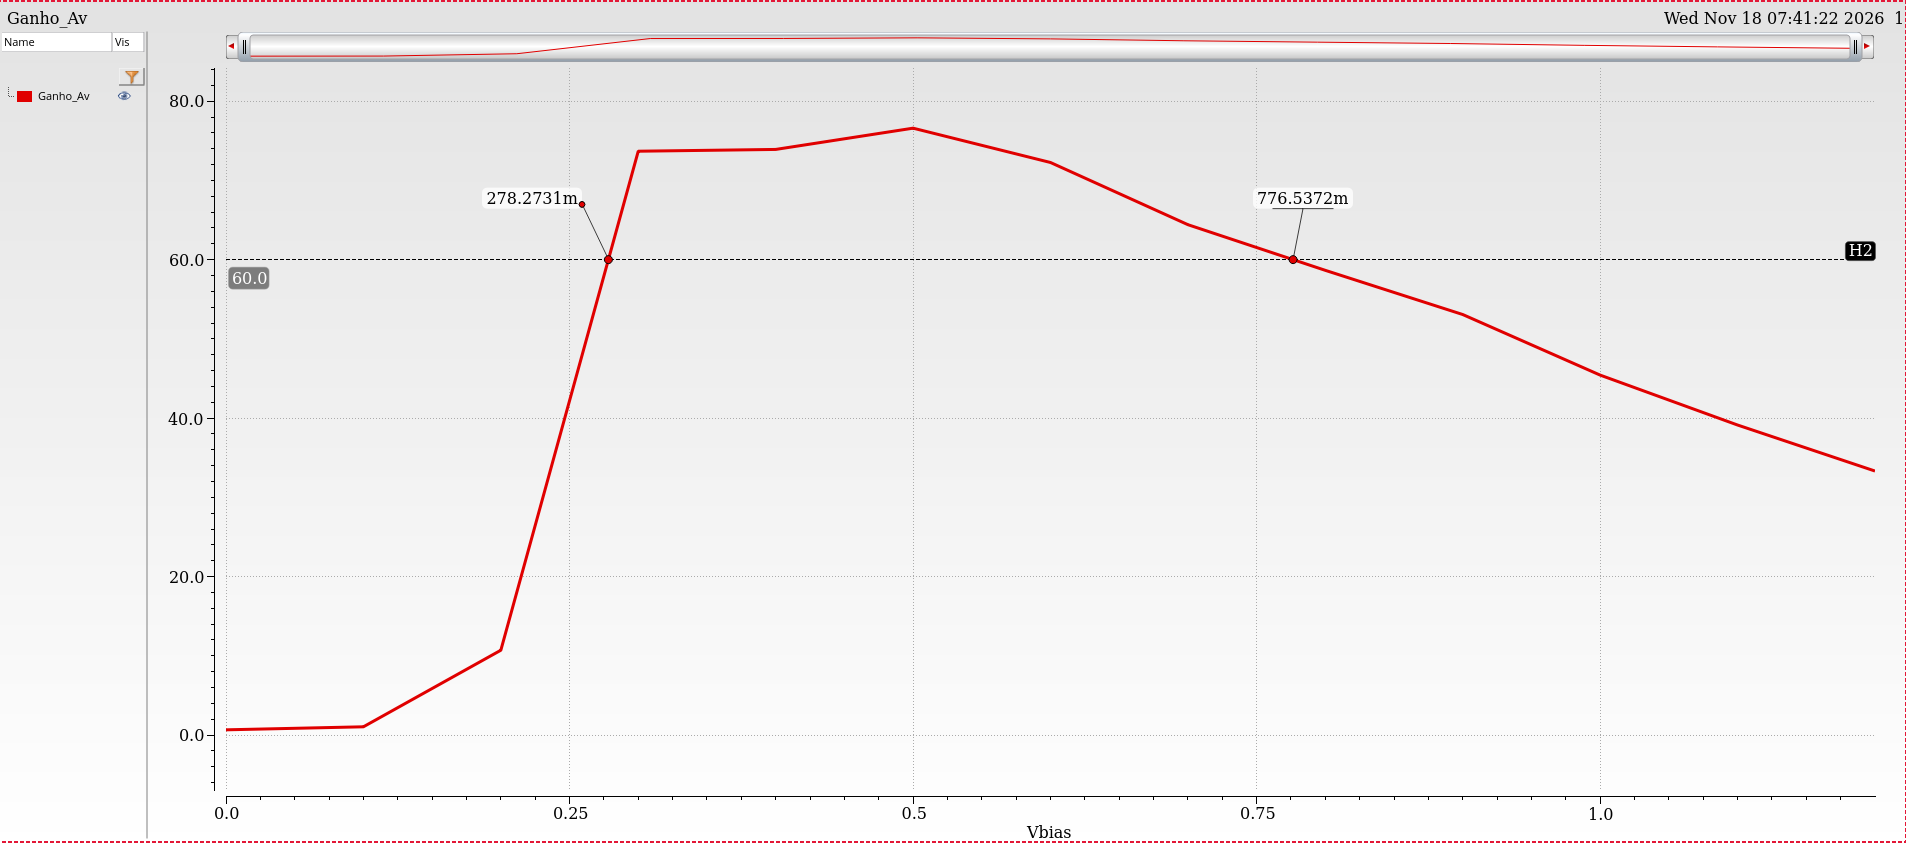
\includegraphics[width=0.80\textwidth]{Geral/Fig/varredura_0_1200m.png}
    \caption{Varredura paramétrica ampla de $V_{Bias}$ ($0$ a $1200\text{ mV}$) mostrando os dois pontos de cruzamento para $|A_{vo}| = 60\text{ V/V}$.}
    \label{fig:varredura_geral}
\end{figure}

\begin{figure}[H]
    \centering
    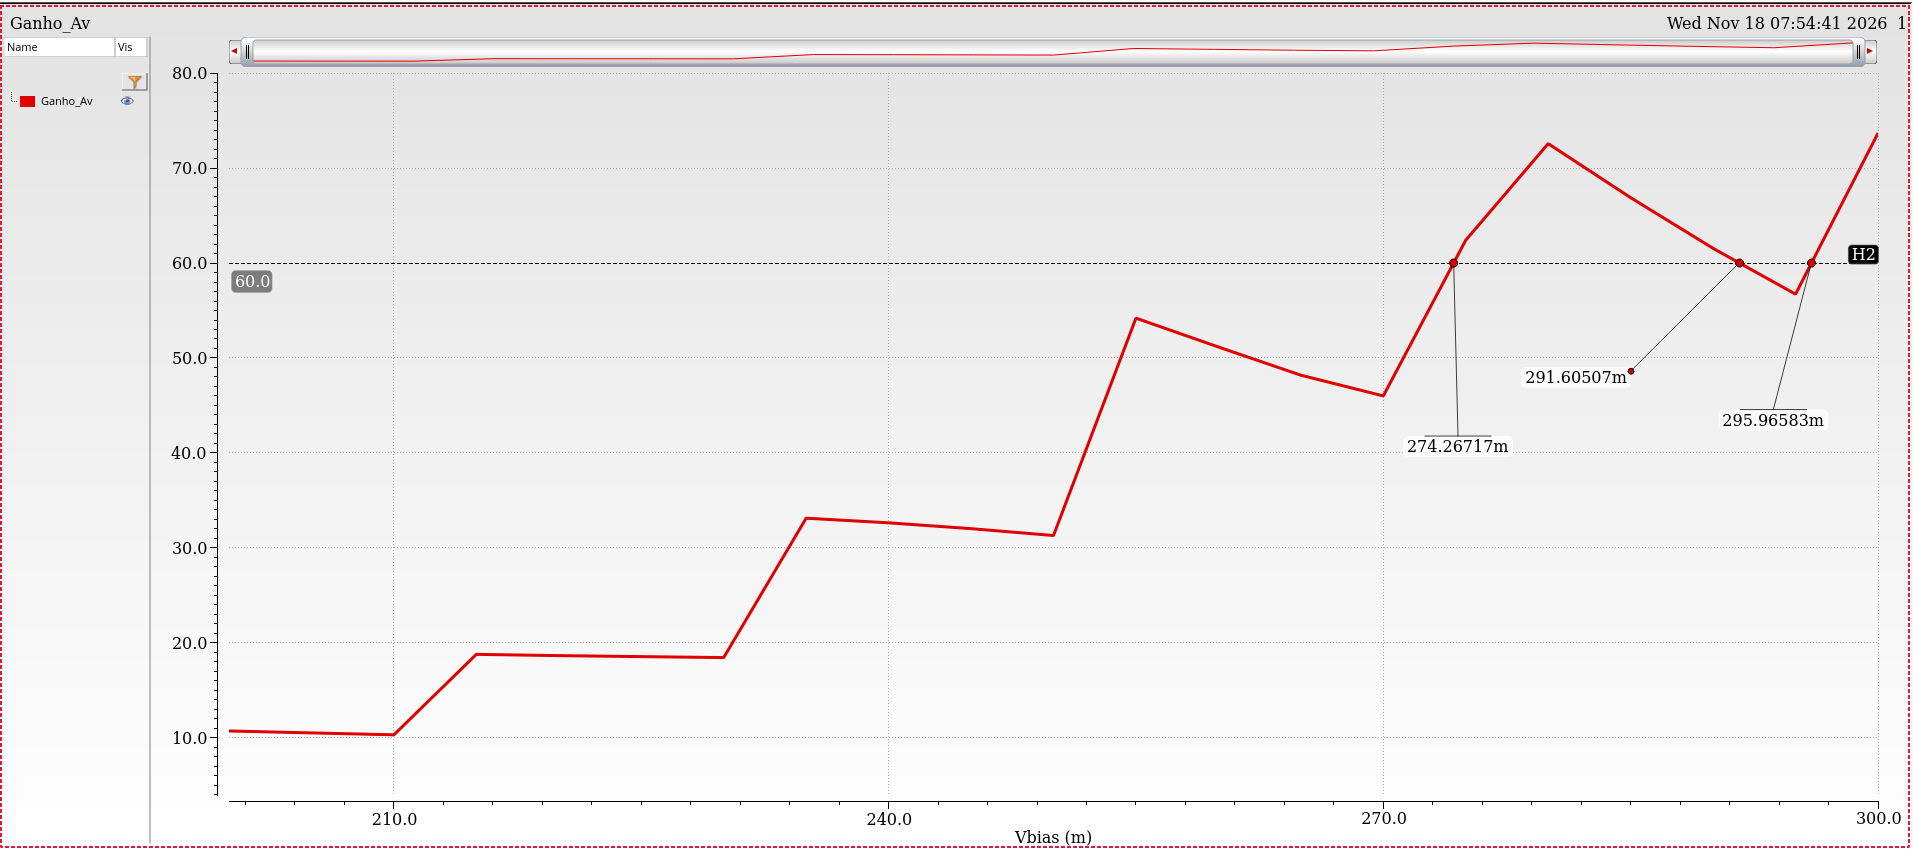
\includegraphics[width=0.80\textwidth]{Geral/Fig/varredura_200_300m.png}
    \caption{Detalhe da varredura de $V_{Bias}$ entre $200\text{ mV}$ e $300\text{ mV}$, evidenciando as oscilações numéricas na região de inversão fraca.}
    \label{fig:varredura_inferior}
\end{figure}

\begin{figure}[H]
    \centering
    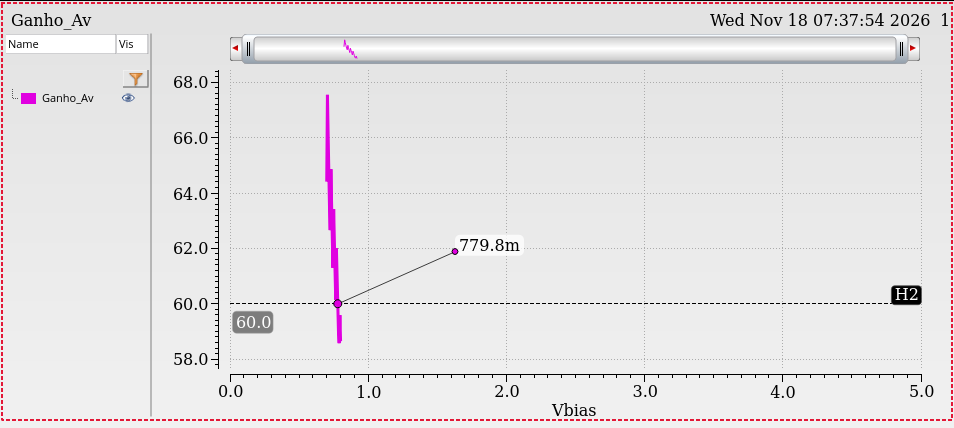
\includegraphics[width=0.80\textwidth]{Geral/Fig/varredura_700_800m.png}
    \caption{Varredura fina de $V_{Bias}$ na faixa superior para determinação exata do ponto de $|A_{vo}| = 60\text{ V/V}$.}
    \label{fig:varredura_fina}
\end{figure}

\paragraph{Conclusão}
\vspace{0.2cm}
Adotou-se a tensão de polarização $V_{Bias} = 779.8\text{ mV}$ ($\approx 777\text{ mV}$ a $780\text{ mV}$), pois nesse ponto o dispositivo opera plenamente em \textbf{saturação (inversão forte)}, superando com folga a tensão de limiar do NMOS ($V_{th} \approx 0.4\text{ V}$). Ao contrário da região inferior de sublimiar (onde a corrente de dreno quase nula provoca atraso na acomodação transitória e imprecisões numéricas), a polarização em $779.8\text{ mV}$ garante canal plenamente formado, resposta linear estável, elevada transcondutância ($g_m$) e o cumprimento da restrição $0 < V_{Bias} \le V_{DD}$.

\subsubsection{Item 1.d -- Transcondutância em Curto-Circuito ($G_m$) e Comparação com o Ponto DC}

\paragraph{Metodologia}
\vspace{0.2cm}
Mantendo $V_{Bias} = 779.8\text{ mV}$, curto-circuitou-se a saída do amplificador conectando o terminal direito de $C_{out}$ diretamente ao terra ($v_{out} = 0\text{ V}$). Executou-se a simulação transiente (\texttt{tran}) para registrar as formas de onda temporais da corrente AC de curto-circuito ($i_{out}$, em $\mu\text{A}$) e da tensão de porta ($v_{in}$, em $\text{mV}$), separando-as em dois painéis no visualizador ViVA e gerando o gráfico de transferência $I \times V$ (\texttt{Iout\_Vin}) via função \textit{Y vs Y} (\texttt{IT("/Cout/MINUS")} no eixo Y em função de \texttt{VT("/Vin")} no eixo X) para extração gráfica do coeficiente angular via marcador diferencial.

Para a extração automatizada no Cadence ADE Explorer, configuraram-se as expressões listadas na Tabela~\ref{tab:expressoes_ade}, mantendo preservadas (porém desativadas) as expressões de tensão da etapa anterior (\texttt{Ganho\_Av} e \texttt{Av\_Inst}) e ativando as equações de curto-circuito (\texttt{Gm\_Tran} e \texttt{ro\_tran}) e de ponto de operação estático (\texttt{gm\_dc} e \texttt{ro\_dc}) obtidas mediante simulação \texttt{dc} com \textit{Save DC Operating Point} habilitado sobre o transistor \texttt{nmos\_rf} (\texttt{M0}).

\begin{table}[H]
    \centering
    \caption{Expressões configuradas no Cadence ADE Explorer nas etapas de ensaio do estágio NMOS.}
    \label{tab:expressoes_ade}
    \small
    \begin{tabular}{l l p{7.4cm}}
        \hline
        \textbf{Nome} & \textbf{Etapa do Ensaio} & \textbf{Expressão (\textit{Details})} \\
        \hline
        \texttt{Ganho\_Av} & Aberto / Carga $R_L$ & \texttt{peakToPeak(clip(VT("/Vout") 2e-06 5e-06)) / peakToPeak(clip(VT("/Vin") 2e-06 5e-06))} \\
        \texttt{Av\_Inst} & Aberto / Carga $R_L$ & \texttt{VT("/Vout") / VT("/Vin")} \\
        \texttt{Gm\_Tran} & Curto-Circuito & \texttt{peakToPeak(clip(IT("/Cout/MINUS") 2e-06 5e-06)) / peakToPeak(clip(VT("/Vin") 2e-06 5e-06))} \\
        \texttt{ro\_tran} & Curto-Circuito & \texttt{60 / Gm\_Tran} \\
        \texttt{gm\_dc} & Ponto DC & \texttt{OP("/M0" "gm")} \\
        \texttt{ro\_dc} & Ponto DC & \texttt{1 / OP("/M0" "gds")} \\
        \hline
    \end{tabular}
\end{table}

\paragraph{Resultados}
\vspace{0.2cm}
Conforme observado no gráfico à direita da Figura~\ref{fig:transiente_gm_nmos}, a característica de transferência $i_{out} \times v_{in}$ (\texttt{Iout\_Vin}) apresenta comportamento estritamente linear, cujo coeficiente angular fornece diretamente o módulo da transcondutância em curto-circuito ($|G_m|$), apresentando inclinação positiva de $+10.26\text{ mA/V}$ devido à convenção do terminal de saída do capacitor (\texttt{IT("/Cout/MINUS")}, corrente fluindo do capacitor para o terra). Por meio da ferramenta de marcador diferencial (\textit{Delta Marker}) do Cadence ViVA ($\Delta v_{in} = 755.79\ \mu\text{V}$ e $\Delta i_{out} = 7.756\ \mu\text{A}$), extraiu-se $|G_m| = 10.2626\text{ mA/V}$ ($\approx 10.26\text{ mS}$), valor confirmado exatamente pela expressão \texttt{Gm\_Tran} avaliada na Calculator:
\begin{equation}
    |G_m| = \left.\frac{i_{out}}{v_{in}}\right|_{v_{out}=0} = 10.26\text{ mS}
\end{equation}

\begin{figure}[H]
    \centering
    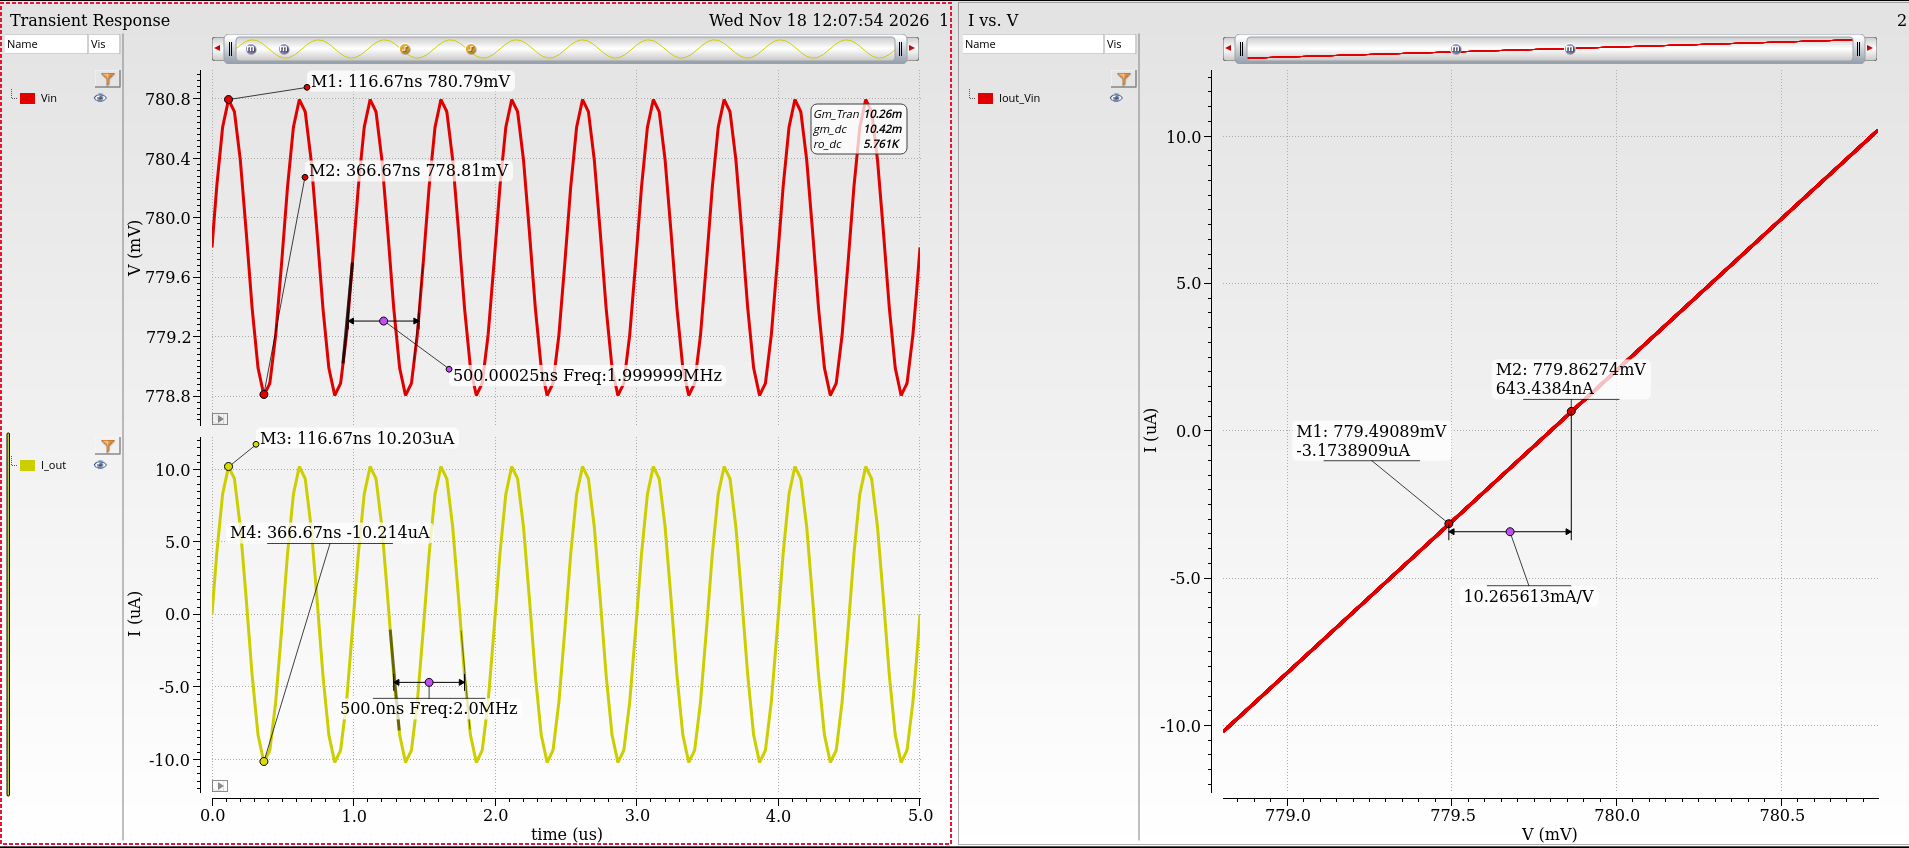
\includegraphics[width=0.92\textwidth]{Geral/Fig/transiente_gm_nmos.png}
    \caption{À esquerda: formas de onda transientes de $v_{in}$ e $i_{out}$ em curto-circuito para $V_{Bias} = 779.8\text{ mV}$. À direita: característica de transferência $i_{out} \times v_{in}$ (\texttt{Iout\_Vin}) linear com coeficiente angular de $10.26\text{ mA/V}$.}
    \label{fig:transiente_gm_nmos}
\end{figure}

Como os passivos são ideais em $2\text{ MHz}$, tem-se $g_m \approx |G_m| = 10.26\text{ mS}$, e a resistência de saída intrínseca calculada via \texttt{ro\_tran} resulta em:
\begin{equation}
    r_{o,\text{tran}} = \frac{|A_{vo}|}{|G_m|} = \frac{60}{10.26\text{ mS}} = 5.845\text{ k}\Omega
\end{equation}
Na análise de ponto de operação DC sobre \texttt{M0}, extraíram-se $g_{m,\text{DC}} = 10.42\text{ mS}$ e $r_{o,\text{DC}} = 1/g_{ds} = 5.761\text{ k}\Omega$. A Tabela~\ref{tab:comparacao_nmos} sintetiza a comparação entre os dois métodos.

\begin{table}[H]
    \centering
    \caption{Comparação entre os parâmetros de pequenos sinais extraídos via transiente e ponto de operação DC para o estágio NMOS.}
    \label{tab:comparacao_nmos}
    \begin{tabular}{lccc}
        \hline
        \textbf{Parâmetro} & \textbf{Simulação Transiente} & \textbf{Ponto de Operação DC} & \textbf{Desvio Relativo} \\
        \hline
        Transcondutância ($g_m$) & $10.26\text{ mS}$ & $10.42\text{ mS}$ & $1.54\%$ \\
        Resistência de saída ($r_o$) & $5.845\text{ k}\Omega$ & $5.761\text{ k}\Omega$ & $1.46\%$ \\
        \hline
    \end{tabular}
\end{table}

\paragraph{Conclusão}
\vspace{0.2cm}
A excelente concordância entre os parâmetros extraídos no domínio do tempo e no ponto de operação DC (desvios relativos inferiores a $1.6\%$) comprova que a excitação de $1\text{ mV}$ mantém o transistor em regime estritamente linear de pequenos sinais, conforme evidenciado pela reta na curva $i_{out} \times v_{in}$, e valida o dimensionamento dos elementos passivos adotados em $2\text{ MHz}$.



\subsection{Questão 2 -- Amplificador Fonte-Comum com Transistor PMOS}

\subsubsection{Item 2.a -- Esquemático Proposto e Dimensionamento Passivo}

O esquemático do estágio amplificador fonte-comum utilizando transistor PMOS está representado na Figura~\ref{fig:esquematico_pmos}.

\begin{figure}[H]
    \centering
    \begin{circuitikz}[american voltages, line width=1.1pt]
        \ctikzset{tripoles/mos style/arrows}
        
        % --- Transistor PMOS invertido verticalmente (Source em cima, Drain em baixo) ---
        \draw (6,2.2) node[pmos](M1){};
        % Garante ligação do bulk ao source (nó superior)
        
        % --- Malha de Entrada (a cinza: v_Sig com + em cima e R_Sig) ---
        \draw[black] (0,2.2) to[V, l=${v_{Sig}}$, color=black] (0,0) node[ground]{};
        \draw[black] (0,2.2) to[R, l=${\mathcal{R}_{Sig}}$, color=black] (1.8,2.2);

        % --- Capacitor Cin e Terminal v_in (azul) ---
        \draw (1.8,2.2) to[C] (3.4,2.2) -- (6,2.2);
        \draw (3.4,2.2) -- (3.4,2.9) node[ocirc, label={[blue]above:\large $v_{in}$}]{};

        % --- Indutor Lin e barra V_Bias ---
        \draw (4.7,2.2) to[L] (4.7,4.6);
        \draw (4.1,4.6) -- (5.3,4.6) node[midway, above]{$\text{V}_{\text{Bias}}$};

        % --- Indutor Lout e barra V_DD (alinhados exatamente com M1.S) ---
        \draw (M1.S) -- (M1.S |- 0,3.2) to[L] (M1.S |- 0,5.2);
        \draw ($(M1.S |- 0,5.2)+(-0.6,0)$) -- ($(M1.S |- 0,5.2)+(0.6,0)$) node[midway, above]{$\text{V}_{\text{DD}}$};

        % --- Ligação do Dreno ao Terra (alinhada com M1.D) ---
        \draw (M1.D) -- (M1.D |- 0,0) node[ground]{};

        % --- Saída: Capacitor Cout, Carga RL (cinza) e Terminal v_out (azul) ---
        \coordinate (outNode) at (M1.S |- 0,3.1);
        \draw (outNode) to[C] ($(outNode)+(2.0,0)$) -- ($(outNode)+(3.4,0)$)
            node[ocirc, label={[blue]above:\large $v_{out}$}]{};
        \draw[black] ($(outNode)+(2.3,0)$) to[R, l=${\mathcal{R}_L}$, color=black] ($(outNode)+(2.3,-2.4)$)
            node[ground, color=black]{};
    \end{circuitikz}
    \caption{Esquemático do amplificador fonte-comum com transistor PMOS.}
    \label{fig:esquematico_pmos}
\end{figure}

% =================================================================
% SEÇÃO DE PERGUNTAS DO ROTEIRO
% =================================================================
\section{Perguntas}
import numpy as np

# ==========================================
# 1. PARÂMETROS DO CIRCUITO (f = 2 MHz)
# ==========================================
f = 2e6                  # Frequência de operação (2 MHz)
w = 2 * np.pi * f        # Frequência angular (rad/s)

R_sig = 50.0             # Resistência da fonte de sinal (Ohms)
R_L = 2000.0             # Resistência de carga no item 1.b (Ohms)
gm = 8.42e-3             # Transcondutância do NMOS (A/V)
ro = 25e3                # Resistência de saída intrínseca do NMOS (Ohms)

# ==========================================
# 2. DIMENSIONAMENTO ANALÍTICO (MARGEM >= 99% DO GANHO)
# ==========================================
# Critério: X_C <= R / fator  e  X_L >= fator * R
Cin_min = 10 / (w * R_sig)          # X_Cin <= 5 Ohms
Lin_min = (100 * R_sig) / w         # X_Lin >= 5 kOhms
Cout_min = 100 / (w * R_L)          # X_Cout <= 20 Ohms
Lout_min_RL = (100 * R_L) / w       # Para operação com RL = 2 kOhms
Lout_min_aberto = (50 * ro) / w     # Para operação em aberto (item 1.c, sem RL)

print("=== VALORES MÍNIMOS CALCULADOS (f = 2 MHz) ===")
print(f"Cin  mínimo : {Cin_min*1e9:.2f} nF  -> Sugerido: 100 nF a 1 uF")
print(f"Cout mínimo : {Cout_min*1e9:.2f} nF  -> Sugerido: 100 nF a 1 uF")
print(f"Lin  mínimo : {Lin_min*1e3:.2f} mH  -> Sugerido: 1 mH a 10 mH")
print(f"Lout mínimo (com RL)   : {Lout_min_RL*1e3:.2f} mH -> Sugerido: 20 mH")
print(f"Lout mínimo (sem RL)   : {Lout_min_aberto*1e3:.2f} mH -> Sugerido: 100 mH\n")

# ==========================================
# 3. VERIFICAÇÃO DO GANHO EXATO COM OS VALORES ESCOLHIDOS
# ==========================================
def calcular_ganho(Cin, Cout, Lin, Lout, RL=R_L, gm_val=gm, ro_val=ro):
    # Impedâncias complexas em j*w
    Z_Cin = 1 / (1j * w * Cin)
    Z_Lin = 1j * w * Lin
    Z_Cout = 1 / (1j * w * Cout)
    Z_Lout = 1j * w * Lout

    # Divisor de tensão na entrada (considerando porta do MOSFET em aberto em 2 MHz)
    H_in = Z_Lin / (R_sig + Z_Cin + Z_Lin)

    # Impedância de carga vista pelo dreno: ro || Lout || (Cout + RL)
    if RL is None or np.isinf(RL):
        # Circuito aberto (item 1.c): dreno vê apenas ro || Lout
        Z_dreno = 1 / (1/ro_val + 1/Z_Lout)
        H_out = 1.0
    else:
        Z_ramo_RL = Z_Cout + RL
        Z_dreno = 1 / (1/ro_val + 1/Z_Lout + 1/Z_ramo_RL)
        H_out = RL / Z_ramo_RL

    Av = -gm_val * Z_dreno * H_in * H_out
    return np.abs(Av)

# Teste com os valores ideais escolhidos no Cadence
Av_ideal_RL = gm * (ro * R_L / (ro + R_L))
Av_sim_RL = calcular_ganho(Cin=1e-6, Cout=1e-6, Lin=10e-3, Lout=100e-3, RL=R_L)

# Teste em circuito aberto (item 1.c, onde gm * ro = 60)
gm_item_c = 60 / ro
Av_sim_aberto = calcular_ganho(Cin=1e-6, Cout=1e-6, Lin=10e-3, Lout=100e-3, RL=np.inf, gm_val=gm_item_c)

print("=== VERIFICAÇÃO DE GANHO ===")
print(f"Ganho teórico assintótico (com RL=2k) : {Av_ideal_RL:.2f} V/V")
print(f"Ganho com C=1u, Lin=10m, Lout=100m    : {Av_sim_RL:.2f} V/V ({Av_sim_RL/Av_ideal_RL*100:.2f}% do ideal)")
print(f"Ganho em aberto (item 1.c, alvo = 60) : {Av_sim_aberto:.2f} V/V")


% --- REFERÊNCIAS BIBLIOGRÁFICAS ---
\bibliographystyle{ieeetr}
\bibliography{referencias}

\end{document}